\documentclass[TS]{sesamanuel}

% commandes utilisées pour la physiques


% divers
\providecommand{\abs}[1]{\lvert#1\rvert}	% pour avoir les valeurs absolues
\providecommand{\norme}[1]{\lVert#1\rVert}	% pour avoir les normes en mode math
\providecommand{\vect}[1]{\overrightarrow{#1}}	% les vecteurs en mode math
\newcommand{\ee}[1]{$\times$10$^{{#1}}$}	% x10^argument
\newcommand{\eem}[1]{\times 10^{{#1}}}		% x10^argument en mode math

% physique : unités
\newcommand{\vit}{\,m$\cdot$s$^{-1}$\xspace} 		% m.s-1
\newcommand{\vitk}{\,km$\cdot$h$^{-1}$\xspace}		% km.h-1
\newcommand{\acc}{\,m$\cdot$s$^{-2}$\xspace} 		% m.s-2
\newcommand{\vitr}{\,rad$\cdot$s$^{-1}$\xspace} 	% rad.s-1

\newcommand{\unitun}[2]{\,{#1}$^{{#2}}$\xspace} 	% arg1^arg2
\newcommand{\unitdeux}[3]{\,{#1}$\cdot${#2}$^{{#3}}$\xspace} % arg1.arg2^arg3
\newcommand{\unittrois}[4]{\,{#1}$\cdot${#2}$\cdot${#3}$^{{#4}}$\xspace} % arg1.arg2.arg3^arg4

% physique : dérivées
\newcommand{\dt}[1]{\frac{\text{d}{#1}}{\text{d}t}}	% en mode math d(arg1)/dt
\newcommand{\ddt}[1]{\frac{\text{d}^2{#1}}{\text{d}t^2}}	% en mode math d2(arg1)/dt2

% physique : vecteur à 2 et à 3 composantes et les accolades pour 2 et 3 lignes
\newcommand{\trinome}[3]{\left(\begin{matrix}{#1}\\{#2}\\{#3}\\ \end{matrix}\right)} %id. binom
\newcommand{\binome}[2]{\left(\begin{matrix}{#1}\\{#2}\\ \end{matrix}\right)} %id. binom
\newcommand{\binacc}[2]{\left\lbrace\begin{array}{l}{#1}\\{#2}\\ \end{array}\right.} % accolade
\newcommand{\trinacc}[3]{\left\lbrace\begin{array}{l}{#1}\\{#2}\\{#3}\\ \end{array}\right.} %ac


% thermodynamique
\newcommand{\jmol}{\,J$\cdot$mol$^{-1}$\xspace} 	% J.mol-1
\newcommand{\kjmol}{\,kJ$\cdot$mol$^{-1}$\xspace} 	% kJ.mol-1
\newcommand{\dhf}[1]{\Delta \text{H}^\text{o}_\text{f}(\text{#1})}  % delta H° formation (X)
\newcommand{\dhfr}{\Delta \text{H}^\text{o}_\text{f}}  % delta H° formation
\newcommand{\dhr}{\Delta \text{H}^\text{o}_\text{R}}  % delta H° réaction
\newcommand{\dho}{\Delta \text{H}^\text{o}}  % delta H°
\newcommand{\dso}{\Delta \text{S}^\text{o}}  % delta S°
\newcommand{\dgo}{\Delta \text{G}^\text{o}}  % delta G°
\newcommand{\dsr}{\Delta \text{S}^\text{o}_\text{R}}  % delta S° réaction

% chimie
\newcommand{\mm}{\,g$\cdot$mol$^{-1}$\xspace} 		% g.mol-1
\newcommand{\conc}{\,mol$\cdot$L$^{-1}$\xspace}	% mol.L-1
\newcommand{\concmass}{\,g$\cdot$L$^{-1}$\xspace}	% g.L-1
\newcommand{\condulambda}{\,S$\cdot$m$^{2}\cdot$mol$^{-1}$\xspace} % S.m2.mol-1


\input{commandes-tikz}

\graphicspath{%
  {forcesEtInteractions/images/}%
  {annexes/images/}%
  {images/}%
}

% création d'un nouveau thème Mécanique pour le document
\NewThema{M}{m}{mécanique}{Mécanique}{MÉCANIQUE}{PartieFonction}{A3}
\renewcommand\ListeMethodesThemes{{m}{M}}


\begin{document}

%%%%%%%%%%%%%%%%%%%%%%%%%%
% 3e de couverture
%%%%%%%%%%%%%%%%%%%%%%%%%%
\newpage

\begin{prerequis}[Un manuel Florimont]
\begin{itemize}
\item L'Institut Florimont a réalisé la transcription dans le langage de description de documents libre et gratuit \LaTeX{} en utilisant la classe \texttt{sesamanuel} développée par l'association Sésamath;
\item E. Villié a réalisé la couverture pour l'Institut Florimont;
\item Version Septembre 2019 --- Institut Florimont (Genève);
\item Publication sous licence libre Creative Commons CC-BY-SA
\end{itemize}
 \end{prerequis}

\vspace{1em}
%%%%%%%%%%%%%%%%%%%%%%%%%%
% fin de la 3e de couverture
%%%%%%%%%%%%%%%%%%%%%%%%%%

% on règle le numéro de la première page
\setcounter{page}{6}

% et la, premier chapitre du livre
\themaM
\chapter{Forces et interactions}\label{ForcesInteractions}


\activites










\begin{activite}[Modéliser une situation physique : système et objets]

Lorsqu'on étudie une situation physique dans laquelle plusieurs objets sont présents, on doit distinguer un objet en particulier qui nous intéresse. C'est cet objet que l'on étudie : on veut connaître sa position, sa vitesse, comment va évoluer son mouvement, etc. L'objet qu'on étudie est appelé le \textbf{système}.


\begin{minipage}{.48\linewidth}
\textbf{Apprenons à observer une situation} (image ci-contre). Nous sommes intéressé par le mouvement du skieur. Quels sont les objets en présence importants pour comprendre le mouvement du skieur ? Quel est le système étudié ?
\end{minipage}%
\hfill
\begin{minipage}{.48\linewidth}
\centering
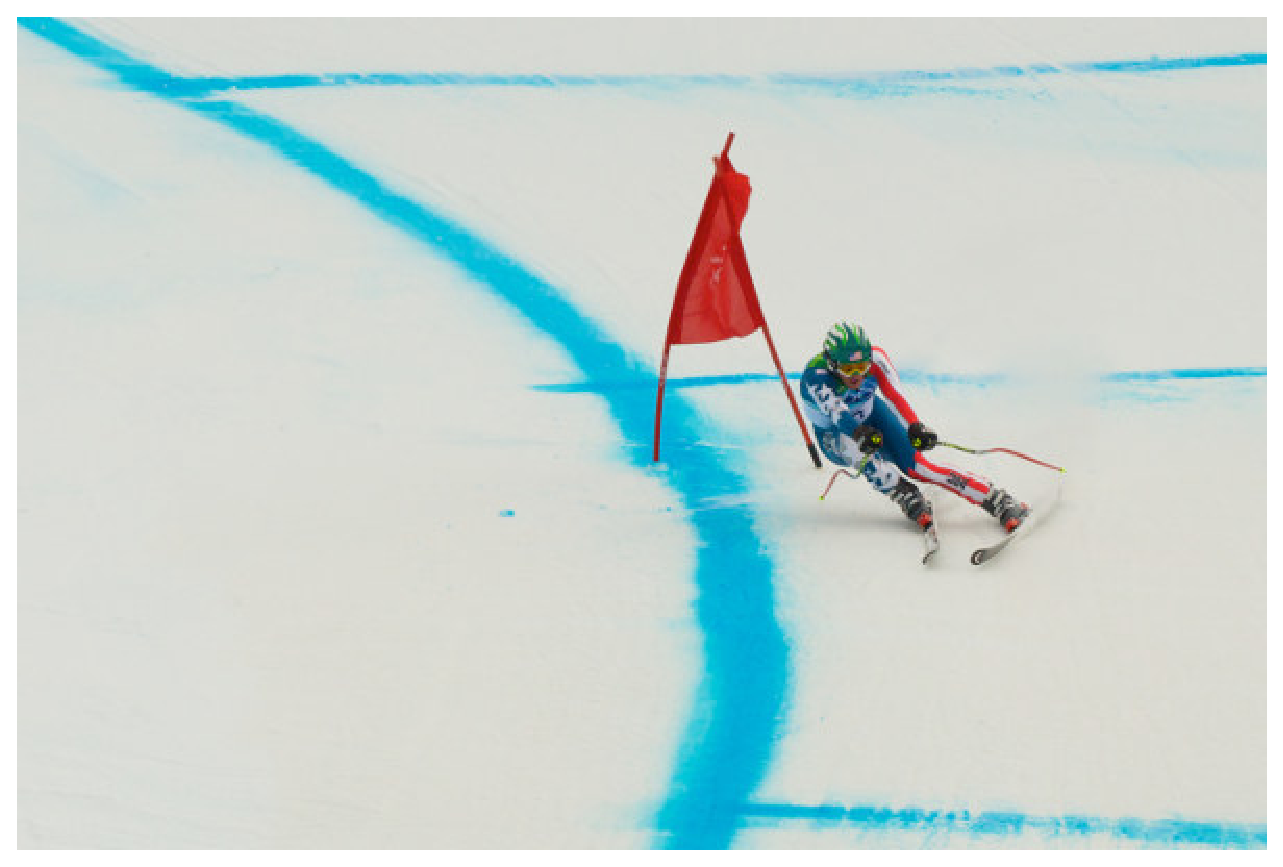
\includegraphics[width=.9\linewidth]{skieur} \\
{\scriptsize \textsl{Source : commons.wikimedia.org}} % https://commons.wikimedia.org/wiki/File:2010_Winter_Olympics_Bode_Miller_in_downhill.jpg#/media/File:2010_Winter_Olympics_Bode_Miller_in_downhill.jpg
\end{minipage}

\end{activite}










\begin{activite}[Action mécanique]


Lorsqu'un objet agit sur un autre objet, on parle d'\textbf{action mécanique}.

Si les deux objets se touchent, on dit qu'il y a \textbf{action mécanique de contact} (exemple : un homme qui pousse une armoire). Par contre, si les deux objets ne se touchent pas, on dit qu'il y a \textbf{action mécanique à distance} (ex : le Soleil qui attire la Terre).   

L'objet qui exerce l'action est appelé \textbf{acteur}. 

\vspace{1em}

\textsl{Voici quatre situations. Après les avoir observées, compléter le tableau suivant, en vous aidant de la question posée pour définir quel objet est l'acteur.}

\vspace{1em}

\begin{minipage}[c]{.2\linewidth}
\centering%
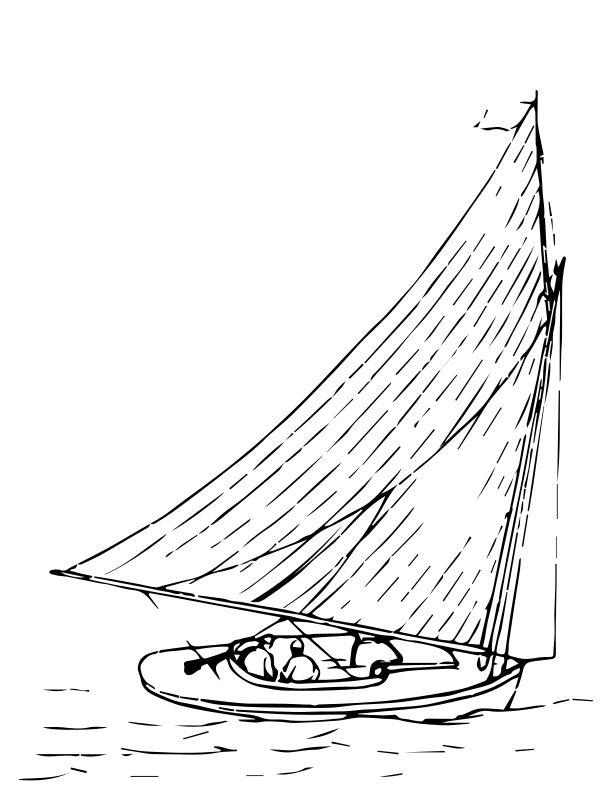
\includegraphics[angle=0,width=.5\linewidth]{bateau} 
% source : openclipart
\end{minipage}\hfill%
\begin{minipage}[c]{.26\linewidth}
\centering%
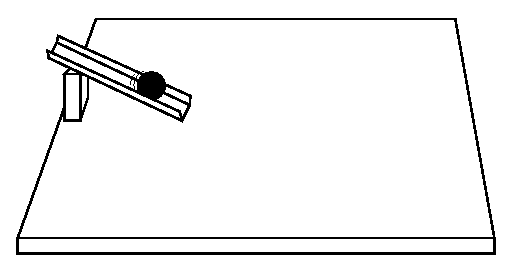
\includegraphics[angle=0,width=.7\linewidth]{billeSeule}
\end{minipage}\hfill%
\begin{minipage}[c]{.26\linewidth}
\centering%
\includegraphics[angle=0,width=.7\linewidth]{billeAimant}
\end{minipage}\hfill%
\begin{minipage}[c]{.2\linewidth}
\centering%
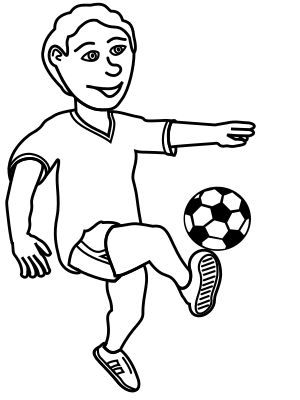
\includegraphics[angle=0,width=.3\linewidth]{footplayer}
% source : openclipart
\end{minipage}\\[.5em]
%
%
\begin{minipage}[c]{.2\linewidth}
\centering
\footnotesize{1 -- Pourquoi le bateau avance-t-il ?}  
\end{minipage}\hfill%
\begin{minipage}[c]{.26\linewidth}
\centering
\footnotesize{2 -- Pourquoi la bille descend-elle ?}
\end{minipage}\hfill%
\begin{minipage}[c]{.26\linewidth}
\centering
\footnotesize{3 -- Pourquoi la bille est-elle déviée ?}
\end{minipage}\hfill%
\begin{minipage}[c]{.2\linewidth}
\centering
\footnotesize{4 -- Pourquoi le ballon monte-t-il en l'air ?}
\end{minipage}

\vspace{1em}

\begin{center}
\renewcommand*\tabularxcolumn[1]{>{\centering\arraybackslash}m{#1}}
\begin{Ctableau}{\linewidth}{5}{c}
\hline
%Situation \no & \multicolumn{1}{c|}{1} & \multicolumn{1}{c|}{2} & \multicolumn{1}{c|}{3} & \multicolumn{1}{c|}{4} \\ \hline
Système & Bateau  & Bille & Bille & Ballon \\ \hline
Action & & & & \\ \hline
Acteur & & & & \\ \hline
Type d'action mécanique & & & & \\ \hline
\end{Ctableau}
\end{center}

\end{activite}

\newpage

\begin{activite}[Modélisation des actions mécaniques]

Les \textbf{actions mécaniques} sont \underline{modélisées} par des \textbf{forces} que l'on \underline{représentent} par un \textbf{vecteur} (donc une \og flèche \fg). Le but est de montrer par ce vecteur l'effet de l'action mécanique sur l'objet étudié.

\vspace{1em}


\begin{minipage}{.58\linewidth}
Voici une situation où un joueur exerce une action mécanique sur un ballon pour le lancer (figure ci-contre). On veut modéliser cette action mécanique par une force.

Quelles informations sont nécessaires pour décrire cette action ?



\end{minipage}%
\hfill
\begin{minipage}{.38\linewidth}
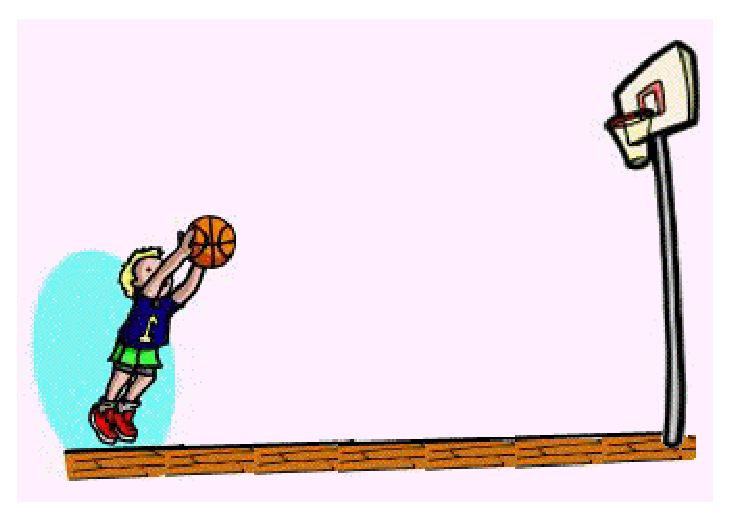
\includegraphics[width=.9\linewidth]{basketShoot}
\end{minipage}

Représenter sur la figure ci-dessus la force qu'exerce le joueur sur la ballon. On donne un nom à cette force, par exemple $\vect{F}_{\text{joueur}/\text{ballon}}$ (qu'on lit \og force du joueur sur le ballon \fg). Ajouter le nom de la force sur la figure.   

\end{activite}




\begin{activite}[Applications]

Pour les deux situations physiques ci-dessous, faire une analyse complète : objets en présence, système, description des actions mécaniques et représentation des forces par des vecteurs.

\vspace{1em}

\begin{minipage}[c]{.48\linewidth}
\centering%
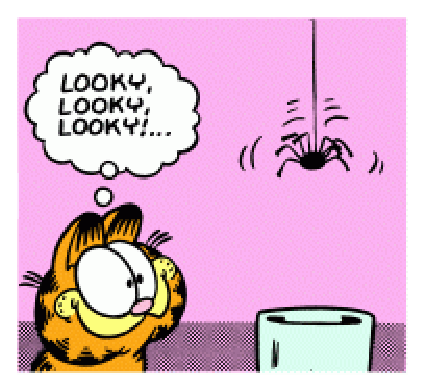
\includegraphics[angle=0,width=.5\linewidth]{garfieldAraignee}
\end{minipage}\hfill%
\begin{minipage}[c]{.48\linewidth}
\centering%
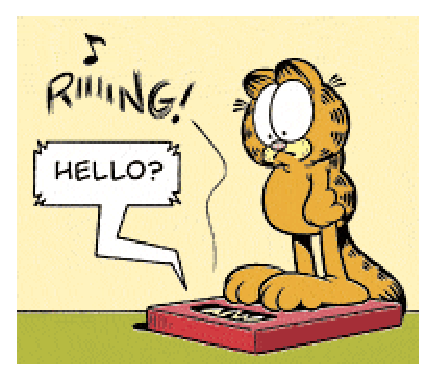
\includegraphics[angle=0,width=.5\linewidth]{garfieldBalance}
\end{minipage}\\[1em]
\begin{minipage}[c]{.48\linewidth}
On s'intéresse au mouvement de l'araignée.
\end{minipage}\hfill%
\begin{minipage}[c]{.48\linewidth}
On s'intéresse au mouvement de Garfield.
\end{minipage}

\end{activite}







\begin{activite}[Situations supplémentaires à étudier]


Pour les situations physiques ci-dessous, faire une analyse complète : objets en présence, système, description des actions mécaniques et représentation des forces par des vecteurs.

\vspace{1em}

\begin{minipage}[c]{.48\linewidth}
\centering%
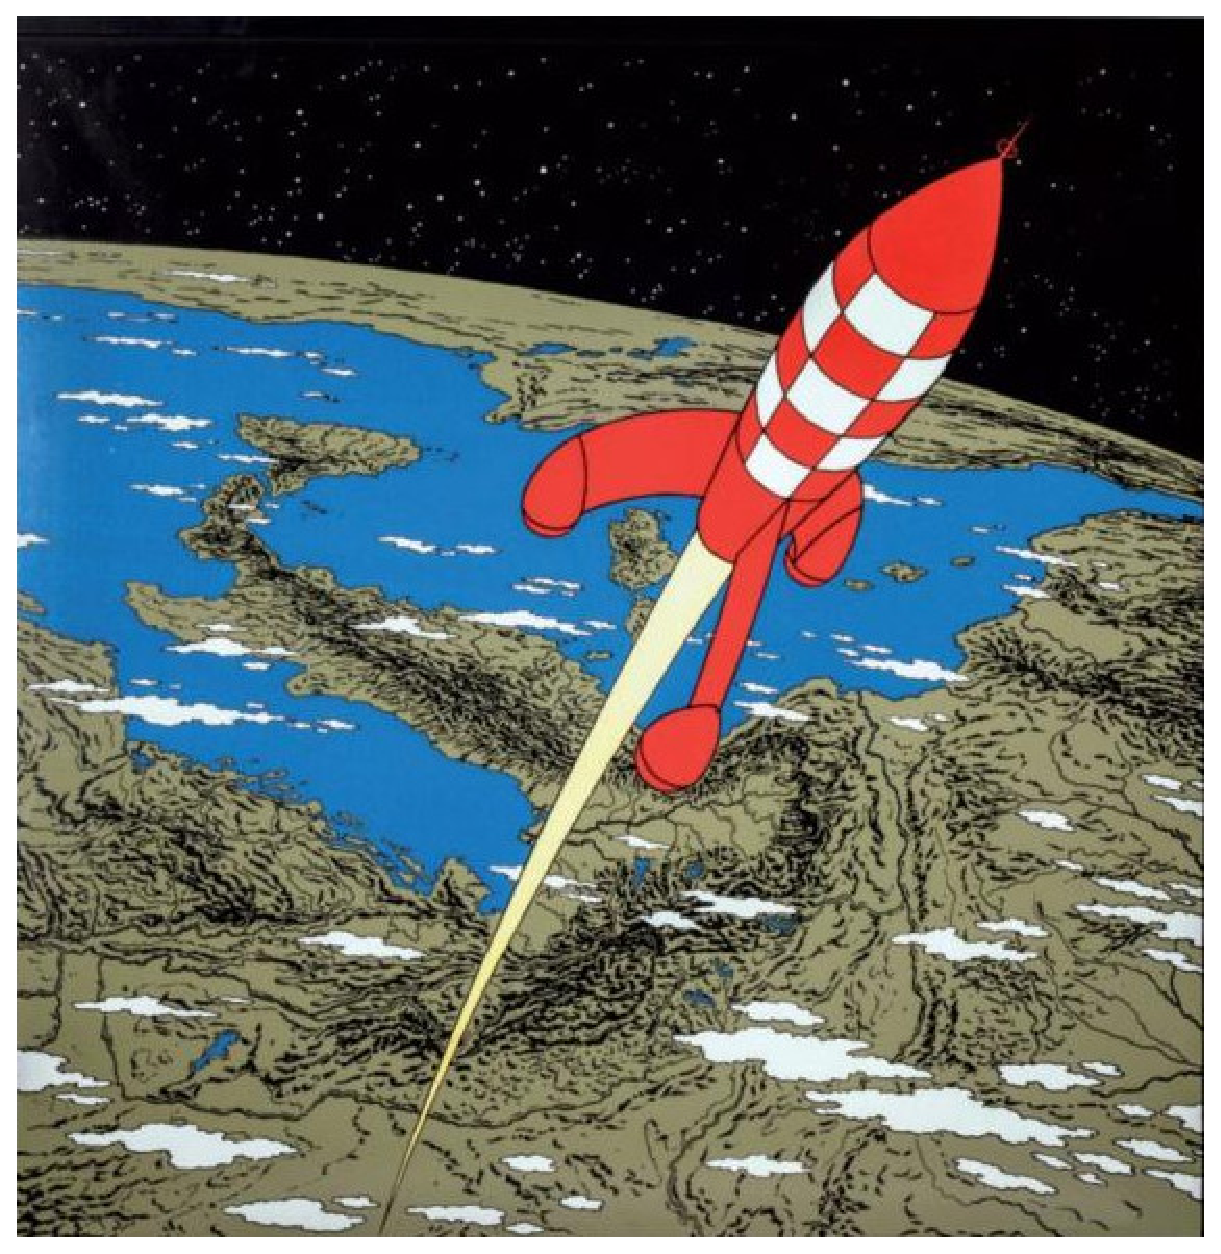
\includegraphics[angle=0,width=.5\textwidth]{tintinFusee}
\end{minipage}\hfill%
\begin{minipage}[c]{.48\linewidth}
On s'intéresse au mouvement de la fusée.
\end{minipage}\\[1em]



\begin{minipage}[c]{.48\linewidth}
\centering%
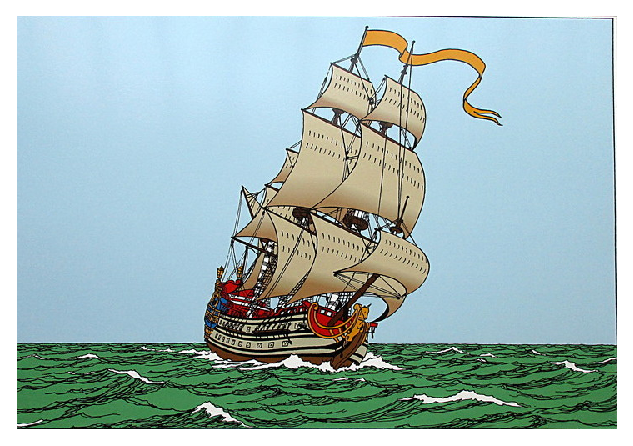
\includegraphics[angle=0,width=.65\textwidth]{tintinBateau}
\end{minipage}\hfill%
\begin{minipage}[c]{.48\linewidth}
On s'intéresse au mouvement du bateau.
\end{minipage}\\[1em]




\begin{minipage}[c]{.48\linewidth}
\centering%
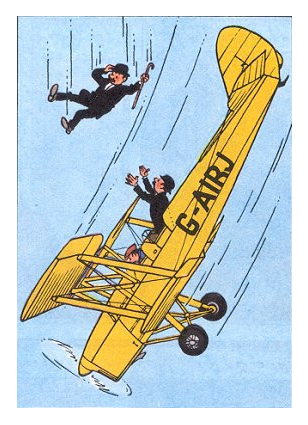
\includegraphics[angle=0,width=.45\textwidth]{tintinAvion}
\end{minipage}\hfill%
\begin{minipage}[c]{.48\linewidth}
On s'intéresse au mouvement de Dupont, puis dans un second temps à celui de l'avion.
\end{minipage}


\end{activite}



\begin{activite}[Les différents types de variables]

\begin{partie}[Les différents types de variables dans une expérience]

Dans une expérience, plusieurs variables entrent en jeu. Il y a toujours une \emph{variable indépendante} et une \emph{variable dépendante}, ainsi qu'un nombre plus ou moins grand de \emph{variables contrôlées}.   

\begin{itemize}
\item \textbf{variable indépendante} : c'est la variable, le paramètre, que l'on fait varier dans l'expérience (cause) ;
\item \textbf{variable dépendante} : c'est la variable, le paramètre, que l'on mesure dans l'expérience après chaque variation de la variable indépendante (effet) ;
\item \textbf{variables contrôlées} : ce sont les variables, les paramètres de l'expérience, qui doivent rester constants afin de ne pas fausser les résultats. 
\end{itemize}

Ainsi, l'expérimentateur modifie la variable indépendante, et regarde comment varie alors la variable dépendante (en la mesurant). Pendant tout le temps de l'expérience, l'expérimentateur vérifie que les variables contrôlées ne sont pas modifiées.
\end{partie}

\begin{partie}[Des cas pratiques pour s'entraîner]

Pour chacune des expériences décrites ci-dessous, identifier les variables indépendante, dépendante et éventuellement contrôlées choisies par l'expérimentateur.

\vspace{1em}

{\footnotesize 

\begin{minipage}[c]{.68\linewidth}
\textbf{Expérience 1 --} On souhaite étudier le lien entre l'intensité de la couleur, notée $A$ et la concentration, notée $C$, d'un sirop à la menthe. Pour cela, on utilise un appareil qui mesure l'intensité de lumière absorbée à travers une cuve contenant une solution de sirop à la menthe. Le but de cette expérience est de montrer que l'intensité de la couleur du sirop est proportionnelle à la concentration en sirop, donc que $A = k \times C$, où $k$ est une constante.
\end{minipage}\hfill%
\begin{minipage}[c]{.28\linewidth}
\centering
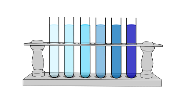
\includegraphics[angle=0,width=.6\linewidth]{echelle-teinte}
\end{minipage}


\vspace{2em}

\begin{minipage}[c]{.68\linewidth}
\textbf{Expérience 2 --}On souhaite étudier le lien entre la chaleur fournie, notée $Q$, à une casserole contenant un litre d'eau, et la variation de température $\Delta T$ de l'eau contenue dans la casserole. Pour cela, on utilise un brûleur à gaz qui permet de connaître la quantité de chaleur transmise, et un thermomètre que l'on place dans l'eau. Le but de cette expérience est de montrer que la température atteinte par l'eau est proportionnelle à la quantité de chaleur fournie, donc que $Q = k \times T$, où $k$ est une constante.
\end{minipage}\hfill%
\begin{minipage}[c]{.28\linewidth}
\centering
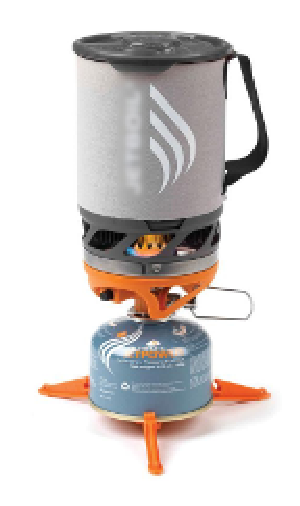
\includegraphics[angle=0,width=.3\textwidth]{jetboil}
\end{minipage}

\vspace{2em}

\begin{minipage}[c]{.68\linewidth}
\textbf{Expérience 3 --} On souhaite étudier le lien entre la tension $U$ aux bornes d'une résistance $R$  et l'intensité $I$ du courant électrique qui la traverse. Pour cela, on dispose d'un circuit électrique où on peut placer une résistance, d'un générateur réglable qui permet de choisir la tension $U$ appliquée aux bornes de la résistance, et d'un ampèremètre pour mesurer l'intensité du courant électrique circulant dans le circuit. Le but de cette expérience est de montrer que la tension aux bornes de la résistance est proportionnelle à l'intensité du courant électrique circulant dans la résistance, donc que $U = R \times I$.
\end{minipage}\hfill%
\begin{minipage}[c]{.28\linewidth}
\centering
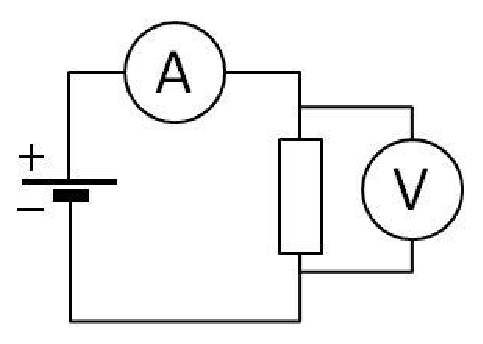
\includegraphics[angle=0,width=.6\linewidth]{resistance}
\end{minipage}

}% fin du footnotesize

\end{partie}
\end{activite}



\TravauxPratiques
\begin{TP}[Balance à élastique]



\begin{cadre}

Le but de ce TP est de trouver la méthode la plus précise permettant de déterminer la masse de deux objets mystères en étirant des élastiques. À vous de concevoir votre manipulation ! Pour cela, il faut suivre les étapes de la fiche méthode \emph{\og Concevoir une expérience \fg} disponible en annexe à la fin de ce manuel.

\end{cadre}

\vspace{1em}



\begin{partie}[Conception et réalisation de l'expérience]

Vous devez concevoir une expérience permettant d'apporter une réponse au problème posé. L'analyse des données recueillies consistera en un graphique représentant l'évolution de la variable dépendante en fonction de la variable indépendante.

Matériel à disposition :
\begin{itemize}
\item élastiques ;
\item support ;
\item boîte de masses marquées ;
\item feuille de papier millimétré.
\end{itemize}

\end{partie}

\vspace{1em}

\begin{partie}[Détermination de la masse des deux objets mystères]

Lorsque vous êtes prêt, appelez le professeur pour déterminer la masse des deux objets mystères !

Matériel à disposition :
\begin{itemize}
\item élastiques ;
\item support ;
\item résultats de l'étape 1.
\end{itemize}

\end{partie}

\vspace{3em}

\textbf{Évaluation}

\vspace{1em}

Vous devez rendre un compte rendu expliquant la démarche suivie, donnant vos résultats et leur analyse. Vous devez expliquez comment vous avez pu déterminer la masse des objets mystères à l'aide de vos résultats.

\vspace{1em}

Grille d'évaluation du compte rendu :
\begin{itemize}
\item les 5 étapes de la démarche scientifique apparaissent et sont correctement développées ;
\item variables choisies (description indépendante, dépendante, et unités) ;
\item protocole détaillé de l'expérience réalisée ;
\item schéma légendé du montage utilisé ;
\item données récoltées (volume, gamme, répartition, tableau de valeur, unités) ;
\item traitement des données (graphique : titre, axes, grandeurs, unités, échelle, qualité, propreté, justesse) ;
\item détermination de la masse des objets mystères et explication de la méthode utilisée ;
\item globalisation (soin, propreté, investissement, qualité générale).
\end{itemize}





\end{TP}


\cours
\begin{cadre}
Souvent, les situations que l'on veut étudier en physique sont complexes. Imaginons un skieur qui descend une piste : ses deux skis glissent sur la neige, le poids de son corps est réparti inégalement sur les deux skis, l'air le freine, la piste n'est pas parfaitement lisse, etc. Si l'on veut pouvoir étudier le mouvement du skieur (notre \emph{objet} d'étude), il faut être capable de simplifier au maximum la situation, mais pas trop ! Il faut donc \emph{négliger} tout ce qu'il n'est pas utile de prendre en compte. Par exemple on peut négliger le frottement des skis sur la neige en faisant la supposition que la glisse est parfaite et que les frottements de l'air sont bien plus forts que les frottements ski--neige. De même, le skieur et son matériel pourront être assimilé à un point unique dont la masse est celle du skieur et de son équipement. Le poids du skieur, qui est réparti sur l'ensemble de la surface des skis, pourra alors être supposé appliqué uniquement sur ce point, etc. C'est ce qu'on appelle \emph{modéliser} la situation : il faut parvenir à la situation la plus simple possible qui corresponde encore suffisamment à la réalité.  

\vspace{.5em}

Voilà le rôle du physicien : à partir d'un objet dans une situation complexe, il doit trouver une modélisation qui corresponde suffisamment à la réalité pour pouvoir prévoir l'évolution du mouvement de l'objet étudié. Au fil des deux premiers chapitres, nous allons apprendre à modéliser une situation physique pour pouvoir l'étudier et prédire comment va varier son mouvement. Ce premier chapitre s'attelle à la modélisation de l'action mécanique.

\vspace{.5em}

Dans un second temps il sera question de la modélisation d'une situation physique à l'aide d'un diagramme objets-interactions qui, comme son nom l'indique, regroupe sur un même diagramme tous les objets en présence et toutes les interactions entre ces objets et un objet particulier : le système étudié. Ce sera également l'occasion de dresser une liste des différentes forces (interactions) que nous allons rencontrer cette année.
\end{cadre}

\section{Introduction}

Ce premier chapitre, où il est question de forces et d'interactions, fait partie de la \emph{mécanique}. 

\textsl{La mécanique (du grec ancien « l'art de construire une machine ») est une branche de la physique dont l'objet est l'étude du mouvement, des déformations ou des états d'équilibre des systèmes physiques. Cette science vise ainsi à décrire les mouvements de différentes sortes de corps, depuis les particules subatomiques avec la mécanique quantique, jusqu'aux galaxies avec la mécanique céleste.}\hfill{\footnotesize(Définition de Wikipedia)}

\section{L'objet étudié : le système}

Lorsqu'on étudie une situation physique dans laquelle plusieurs objets sont présents, on doit distinguer un objet en particulier qui nous intéresse. C'est cet objet que l'on étudie : on veut connaître sa position, sa vitesse, comment va évoluer son mouvement, etc. L'objet qu'on étudie est appelé le \textbf{\MotDefinition{système}{}}. Pour le distinguer, on le note entre accolades, par exemple : \{skieur\}.


\section{Modélisation de l'objet étudié}

Les objets que l'on étudie sont modélisés par un unique point, dont la masse est celui de l'objet. Ce point n'est pas choisi au hasard : c'est le centre de gravité de l'objet.

\begin{center}
    \includegraphics[width=.5\linewidth]{cdg}
\end{center}



\section{Action mécanique}

Lorsqu'un objet agit sur un autre objet, on parle d'\textbf{\MotDefinition{action mécanique}{}}.

Si les deux objets se touchent, on dit qu'il y a \textbf{action mécanique de contact} (exemple : un homme qui pousse une armoire). Par contre, si les deux objets ne se touchent pas, on dit qu'il y a \textbf{action mécanique à distance} (ex : un aimant qui attire un morceau de fer).   

\begin{aconnaitre}[Action mécanique]
Une \textbf{action mécanique}, exercée par un objet (l'acteur) sur un autre objet (le receveur, ici le système), peut :
\begin{itemize}
\item mettre en mouvement le système ;
\item modifier la trajectoire du système ;
\item déformer le système.
\end{itemize}

\vspace{.5em}

Plus la masse du système est faible, plus l'action mécanique qu'il subit est efficace.
\end{aconnaitre}

\vspace{1em}

Exemple : avec la même action mécanique, il est aisé de mettre en mouvement une bicyclette, et difficile de mettre en mouvement une voiture.

\section{Modélisation de l'action mécanique : la force}

Les actions mécaniques sont \underline{modélisées} par des \textbf{\MotDefinition{forces}{}} qui montrent de manière simple l'effet de l'action mécanique sur l'objet étudié.

Graphiquement, les forces sont \underline{représentées} par des \textbf{vecteurs}, car ces objets mathématiques possèdent les mêmes caractéristiques que les forces (voir \S\ \ref{ForceVecteur}). 

\vspace{1em}

Exemple de modélisation d'une action mécanique (figure ci-dessous) : la boîte appuie sur la table. On peut modéliser cette action mécanique par un ensemble de forces représentées par des vecteurs (figure à gauche). Mais ce n'est pas simple de travailler avec tous ces petits vecteurs. On préfère alors utiliser la \textbf{résultante} de toutes ces forces : c'est une force unique, égale à la somme de toutes les autres, et qui est appliquée au centre de gravité de l'objet étudié (figure à droite).


\begin{center}
    \includegraphics[width=.6\linewidth]{boiteTable}
\end{center}


Attention : les actions mécaniques ne sont pas des forces ! Les actions mécaniques sont \emph{modélisées} par des forces car c'est plus simple pour les décrire.




\section{Caractéristiques de la force}

Une force se note $\vect{F}$ ou $\vect{F}_\text{acteur/receveur}$ (dans l'exemple ci-dessous, la force exercée par la Terre sur la Lune est notée $\vect{F}_\text{Terre/Lune}$) : elle est représentée par un vecteur auquel on ajoute un point d'application, généralement le centre de gravité de l'objet, ou un point de contact.


\begin{center}
    \includegraphics[width=.4\linewidth]{force}
\end{center}

\vspace{1em}

\begin{aconnaitre}[\MotDefinition{Caractéristiques d'une force}{}]
Une force est caractérisée par :
\begin{itemize}
\item son \textbf{point d'application} (origine du vecteur, ici $B$) ;
\item sa \textbf{droite d'action} ou \emph{direction} (droite support du vecteur, ici $(AB)$) ;
\item son \textbf{sens} (ici de $B$ vers $A$) ;
\item sa \textbf{valeur} ou \textbf{intensité} (c'est la \emph{norme} du vecteur, ici $\norme{\vect{F}_\text{Terre/Lune}}$), dont l'unité est le newton (symbole : N).

Attention, en physique la norme d'un vecteur est notée tout simplement en enlevant la flèche : $\norme{\vect{F}_\text{Terre/Lune}}$ est notée $F_\text{Terre/Lune}$.
\end{itemize}
\end{aconnaitre}

\vspace{1em}


Le \textbf{\MotDefinition{newton}{}} (symbole : N) équivaut à 1\unittrois{kg}{m}{s}{-2} : cela signifie qu'un Newton est la force colinéaire au mouvement qui, appliquée pendant une seconde à un objet d'un kilogramme, est capable d'ajouter (ou de retrancher) un mètre par seconde à sa vitesse.

\vspace{1em}


Cette petite pomme de 100\,g (figure ci-dessous) applique sur la table où elle est posée une force de 1\,N environ (attention, toutes les forces s'appliquant sur la pomme ne sont pas représentées sur cette figure). La force est représentée ci-dessous à l'échelle.

\begin{center}
    \includegraphics[width=.3\linewidth]{pomme}
\end{center}

\vspace{1em}

L'appareil qui mesure l'intensité de la force est le \textbf{\MotDefinition{dynamomètre}{}}. Il est constitué d'un ressort qui se déforme sous l'action de la force exercée. Un curseur indique alors l'intensité de la force à laquelle le dynamomètre est soumis. Figures ci-dessous : à gauche, différents dynamomètres linéaires et à droite, un dynamomètre circulaire.


\begin{center}
    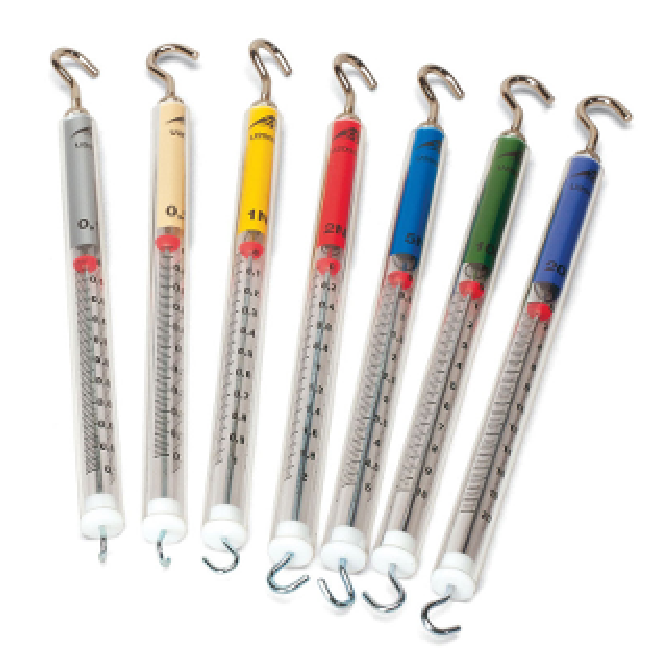
\includegraphics[width=.3\linewidth]{dynamometre}%
    \hfill%
    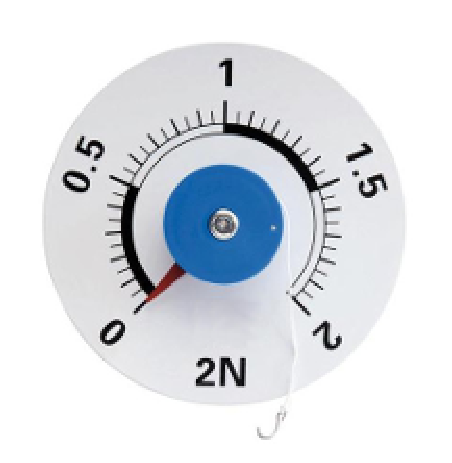
\includegraphics[width=.3\linewidth]{dynamometreRond}
\end{center}



\section{Force et vecteur}\label{ForceVecteur}

\subsection{Rappels sur les vecteurs}

Considérons le vecteur $\vect{AB}$ ci-dessous.

\begin{center}
    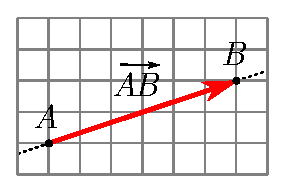
\includegraphics[width=.3\linewidth]{vecteurAB}
\end{center}

\vspace{1em}

Le \MotDefinition{vecteur}{} est un objet mathématique qui contient beaucoup d'informations : une \emph{droite d'action} (\emph{direction} en mathématiques), donnée par la droite passant par le vecteur, dite droite support (ici $(AB)$) ; un \emph{sens}, le long de la droite support (ici de $A$ vers $B$) ; une \emph{intensité} en newton (\emph{norme} en mathématiques), représentée par la taille du vecteur et notée $\norme{\vect{AB}}$.

C'est cet objet qui est utilisé pour représenter les forces en physique, car il contient toutes les informations permettant de les décrire. Le tableau ci-dessous donne la correspondance entre les noms utilisés en physique pour les forces et les propriétés mathématiques du vecteur :

\begin{center}
\renewcommand*\tabularxcolumn[1]{>{\centering\arraybackslash}m{#1}}
\begin{Ltableau}{.8\linewidth}{4}{c}
\hline
\multicolumn{2}{|c|}{\textbf{Vecteur en mathématiques}} & \multicolumn{2}{c|}{\textbf{Force en physique}} \\ \hline
\emph{Nom} & \emph{Notation}& \emph{Nom} & \emph{Notation} \\ \hline
direction & $(AB)$ & \MotDefinition{droite d'action}{} & $(AB)$ \\ \hline
sens & de $A$ vers $B$ & \MotDefinition{sens}{} & de $A$ vers $B$ \\ \hline
norme & $\norme{\vect{AB}}$ & \MotDefinition{intensité}{} (en N) & $AB$\\ \hline
\phantom{point d'application} & & \MotDefinition{point d'application}{} & $A$ \\ \hline
\end{Ltableau}
\end{center}


\begin{methode}[Représenter une force à l'aide d'un vecteur \MethodeRefExercice{representeVecteur}]
\label{methodeForceEchelle}
Pour représenter une force $\vect{T}$ d'intensité 600\,N à l'aide d'un vecteur, il faut choisir une échelle adaptée, par exemple 1\,cm représente 150\,N, puis tracer sur la droite d'action un vecteur de longueur 4\,cm (car $4\times 150=600$) à partir du point d'application.

L'échelle choisie ne doit être ni trop petite ni trop grande. Elle doit permettre au vecteur d'utiliser au mieux l'espace disponible sur la feuille.

\exercice
Représenter la force $\vect{F}$ dont l'intensité est de 625\,N, la droite d'action (MN), le sens de N à M et le point d'application $G$.

\correction
\vspace{.5em}
\begin{tikzpicture}[general]
\draw[quadrillage55] (0,0) grid (7,3);
\pointGraphique{2}{.5}{M}{below left};
\pointGraphique{6}{2.5}{N}{below right};
\pointGraphique{5}{2}{G}{below right};
\end{tikzpicture}
\end{methode}




\subsection{Addition de vecteurs}

Pour additionner deux vecteurs $\vect{u}$ et $\vect{v}$, deux méthodes peuvent être utilisées. Le vecteur somme $\vect{u+v}$ alors obtenu est le même dans les deux cas. 

Considérons les deux vecteurs $\vect{u}$ et $\vect{v}$ ci-dessous.

\begin{center}
    \includegraphics[width=.3\linewidth]{vecteurSomme1}
\end{center}


\begin{methode}[Addition de vecteurs : méthode \og bout à bout \fg \MethodeRefExercice{exAddVect}]
\label{methodeAddBoutBout}

Pour additionner les deux vecteurs $\vect{u}$ et $\vect{v}$, on les place l'un au bout de l'autre. Le vecteur somme $\vect{u+v}$ a pour origine le début du premier vecteur et pour fin l'endroit où se termine le second.

\begin{center}
    \includegraphics[width=.4\linewidth]{vecteurSomme2}
\end{center}

\exercice
En utilisant la méthode bout à bout, faire la somme des vecteurs $\vect{F}$ et $\vect{T}$.

\correction
\vspace{.5em}
\begin{tikzpicture}[general]
\draw[quadrillage55] (0,0) grid (7,3);
\draw[axe] (1,1)--(2,2.5);
\draw[axe] (4,2.5)--(6,1.5);
\draw (1.2,1.7) node[above] {$\vect{F}$};
\draw (5,2) node[above] {$\vect{T}$};
\end{tikzpicture}
\end{methode}


\begin{methode}[Addition de vecteurs : méthode du parallélogramme \MethodeRefExercice{exAddVect}]
\label{methodeAddParall}

Pour additionner les deux vecteurs $\vect{u}$ et $\vect{v}$, on les place de telle sorte qu'ils aient même origine et on trace le parallélogramme ainsi défini (en pointillés sur la figure ci-dessous). La diagonale du parallélogramme correspond au vecteur somme $\vect{u+v}$.

\begin{center}
    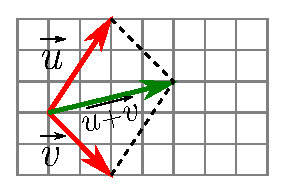
\includegraphics[width=.4\linewidth]{vecteurSomme3}
\end{center}

\exercice
En utilisant la méthode du parallélogramme, faire la somme des vecteurs $\vect{F}$ et $\vect{T}$.
\correction
\vspace{.5em}
\begin{tikzpicture}[general]
\draw[quadrillage55] (0,0) grid (7,3);
\draw[axe] (1,1)--(2,2.5);
\draw[axe] (4,2.5)--(6,1.5);
\draw (1.2,1.7) node[above] {$\vect{F}$};
\draw (5,2) node[above] {$\vect{T}$};
\end{tikzpicture}
\end{methode}



\vspace{2em}

\begin{remarque}
Attention ! Notons bien que $\norme{\vect{u} + \vect{v}} \neq \norme{\vect{u}} + \norme{\vect{v}}$, ce qui est particulièrement trompeur en physique où on écrit $u$ la valeur (norme) du vecteur $\vect{u}$, ce qui donne $(u+v) \neq u + v$... 

C'est ce que montre l'exemple ci-dessous. Les vecteurs $\vect{u}$ et $\vect{v}$ ont pour intensité 2\,N. Le vecteur somme $\vect{u+v}$ a pour intensité 2,8\,N.
\begin{center}
    \begin{tikzpicture}[general]
    \draw[quadrillage55] (0,0) grid (8,3);
    \draw[axe] (1,.5)--(1,2.5); \draw (.5,1.5) node {$\vect{u}$};
    \draw[axe] (2,.5)--(4,.5); \draw (3,1) node {$\vect{v}$};
    \draw[axe] (5,.5)--(7,2.5); \draw (6.5,1) node[above] {$\vect{u+v}$};
    \draw (6,-.25) node {échelle : 2 carreaux $\rightarrow$ 1\,N};
\end{tikzpicture}
\end{center}

\end{remarque}







\section{Résultante des forces}

\begin{aconnaitre}[Résultante d'une force]
Lorsque plusieurs forces sont appliquées sur un même objet, on peut calculer la \textbf{\MotDefinition{résultante des forces}{}}, qui est l'\textbf{addition vectorielle de toutes les forces appliquées} sur l'objet.

\vspace{1em}

\textbf{Tout se passe alors comme si l'objet n'était soumis qu'à la résultante des forces.}


\begin{center}
    \includegraphics[width=.25\linewidth]{resultante1}%
    \hfill%
    \includegraphics[width=.55\linewidth]{resultante2}
\end{center}

{\footnotesize Figure de gauche, la résultante des forces est nulle : tout se passe comme si la voiture n'était soumise à aucune force. Figure de droite, la résultante des forces est non nulle : tout se passe comme si la voiture était soumise à une force dirigée vers la droite : la \emph{force résultante}.}

\end{aconnaitre}












\section{Corde et poulie}


Lorsqu'on applique une force à l'extrémité d'une \textbf{\MotDefinition{corde}{}}, la droite d'action de la force est toujours située le long de la corde. La corde transmet intégralement la force : si on tire avec une force d'intensité 1\,N à l'extrémité de la corde, le dynamomètre va indiquer 1\,N (voir figures ci-dessous).


Une \textbf{\MotDefinition{poulie}{}} ne modifie pas l'intensité d'une force, mais elle permet d'orienter différemment sa droite d'action (voir ci-dessous).

\vspace{1em}

\begin{center}
    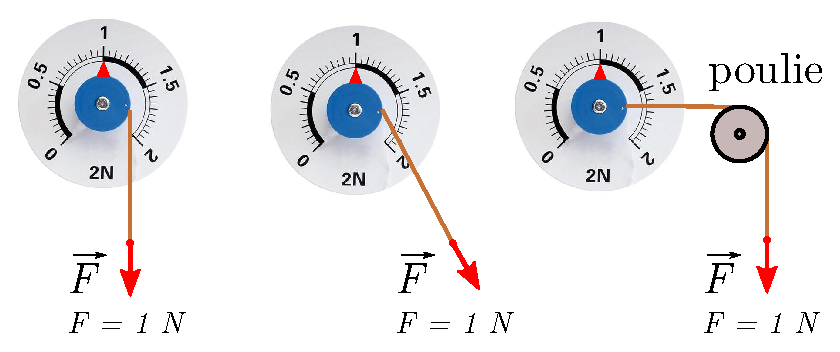
\includegraphics[width=.7\linewidth]{cordePoulie}
\end{center}

\vspace{2em}

\begin{remarque}
notez bien que la force est nommée $\vect{F}$ (grandeur vectorielle), mais que l'intensité de la force est nommée $F$ (grandeur scalaire correspondant à $\norme{\vect{F}}$).
\end{remarque}





\section{Principe des actions réciproques}

Comme montré sur la figure ci-dessous, lorsque le skater pousse le mur avec sa main, alors le mur exerce sur lui une force égale en intensité mais de sens opposé. C'est ce qui permet au skater de se mettre en mouvement vers la droite dans ce cas.

\begin{center}
    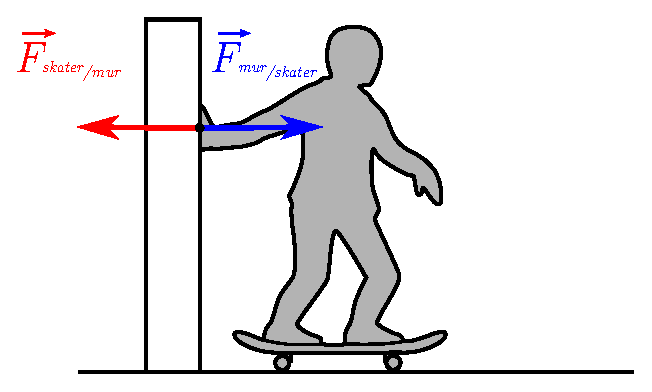
\includegraphics[width=.4\linewidth]{skater}
\end{center}

% il faut ajouter la force du mur sur le skater
% de plus il faut modéliser la situation à côté

Si on étudie le système \{skater\}, il subit de la part du mur la force $\vect{F}_\text{mur/skater}$. La force que le skater applique sur le mur n'est pas une force subie par le système, donc ne nous intéresse pas dans ce cas. 

\vspace{1em}

\begin{aconnaitre}[Principe des \MotDefinition{actions réciproques}{} (3\up{e} loi de Newton)]

Lorsqu'un objet $A$ exerce sur un objet $B$ une force $\vect{F}_{A/B}$, alors l'objet $B$ exerce sur l'objet $A$ une force $\vect{F}_{B/A}$ telle que : {\large\[\vect{F}_{A/B} = -\vect{F}_{B/A}\]}

\begin{center}
    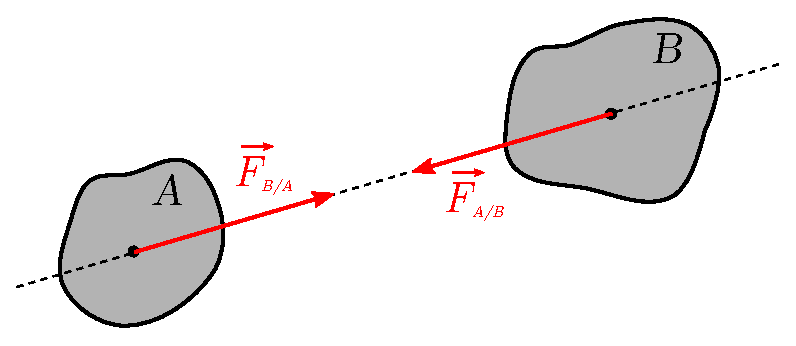
\includegraphics[width=.5\linewidth]{3eLoi}
\end{center}
\end{aconnaitre}
  


\begin{remarque}
lorsqu'un objet applique sur un autre objet une action mécanique, alors celui-ci applique en retour une action mécanique égale mais opposée. Une action mécanique n'existe donc jamais seule et c'est la raison pour laquelle on dit qu'il existe entre deux objets une \textbf{\MotDefinition{interaction}{}} : l'action du premier induit une action en retour du second. 
\end{remarque}


La \textbf{propulsion} repose sur le principe des actions réciproques : comme pour le skater on \og pousse \fg le sol vers l'arrière avec nos pieds afin d'être propulsé vers l'avant : c'est l'action réciproque qui s'exerce sur le système qui le propulse vers l'avant. Et si le sol est verglacé, alors on n'arrive pas à le \og pousser \fg (pas de frottement) et du coup on n'est pas propulsé vers l'avant.

Autres exemples de propulsion : les rames poussent l'eau en arrière pour faire avancer le bateau ; les roues \og pousse \fg la route vers l'arrière afin de faire avancer la voiture ; l'oiseau \og pousse \fg l'air avec ses ailes pour avancer.





\section{Diagramme objets--interactions et modélisation}

Le \MotDefinition{diagramme objets--interactions}{} (DOI) permet de modéliser facilement une situation. Il dresse l'inventaire de tous les objets en interaction avec le système. À chaque interaction mentionnée correspond une force dans la modélisation.

\begin{methode}[Construction d'un diagramme objets--interactions\MethodeRefExercice{doiFirst}]
\label{methodeDOI}

Pour construire un diagramme objets--interactions, il faut :
\begin{enumerate}
\item placer l'objet étudié (le système) dans un rectangle entouré par des traitillés 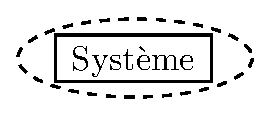
\includegraphics[width=2cm]{DOIsysteme};
\item énumérer tous les objets en interaction avec le système et les représenter dans des rectangles 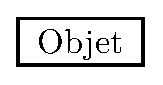
\includegraphics[width=1.2cm]{DOIobjet} ; 
\item représenter par des flèches en trait plein et à deux pointes (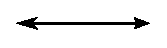
\includegraphics[width=1cm]{DOIflecheP}) les interactions de contact entre les objets et le système ;
\item représenter par des flèches en traitillé et à deux pointes (\includegraphics[width=1cm]{DOIflecheT}) les interactions à distance entre les objets et le système ;
\item auprès de chaque flèche, décrire l'interaction ;
\item ne pas oublier la légende.
\end{enumerate}


\vspace{1em}

Exemple : dans la situation à gauche ci-dessous, on étudie la voiture (arrêtée). À droite, le diagramme objets--interactions correspondant.


\begin{center}
    \includegraphics[width=.4\linewidth]{voiture}%
    \hfill%
    \includegraphics[width=.5\linewidth]{DOIexemple}
\end{center}

\exercice
Construire le diagramme objets-interactions pour un grêlon tombant du ciel (système étudié : le grêlon).
\correction
\vspace{4cm}
\phantom{.}
\end{methode}


\begin{remarque}
lorsque la vitesse d'un objet est faible et/ou que sa masse volumique est largement plus grande que celle de l'air, on néglige l'action de l'air sur le système. C'est le cas dans l'exemple ci-dessus.
\end{remarque}

\vspace{1em}

\begin{aconnaitre}[Du DOI aux forces appliquées au système]
La modélisation d'une situation à partir d'un diagramme objets--interactions est aisée : à chaque interaction mentionnée dans le diagramme objets--interactions correspond une force appliquée au système étudié.
\end{aconnaitre}

\vspace{1em}

Pour l'exemple de la voiture, il y a deux interactions dans le DOI donc le système \{voiture\} est soumis à deux forces appelées ici $\vect{P}$ (le poids) et $\vect{R}$ (la réaction du support) :

\begin{center}
    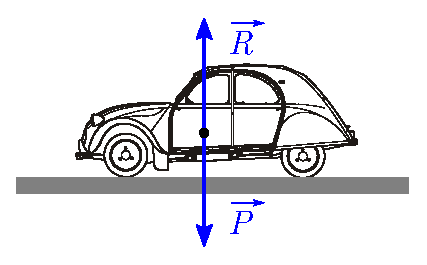
\includegraphics[width=.4\linewidth]{voitureForce}%
    \hfill%
    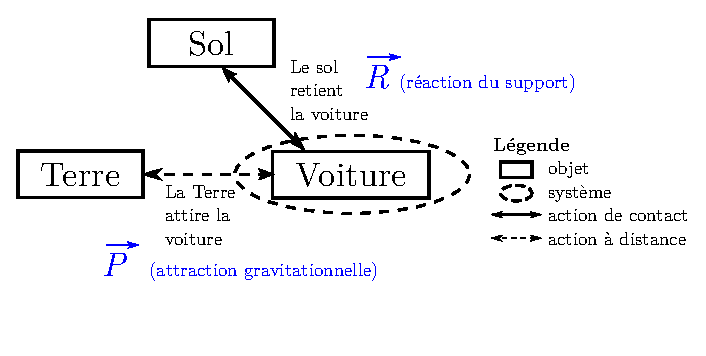
\includegraphics[width=.4\linewidth]{DOIexempleForce}
\end{center}



\begin{aconnaitre}[Le cas de l'air dans les DOI]
La force exercée par l'air sur le système étudé est négligeable devant les autres forces dans deux cas :
\begin{itemize}
    \item le système possède une vitesse nulle ou faible ;
    \item la masse volumique du système est très grande devant celle de l'air.
\end{itemize}

\vspace{.5em}
Ainsi, on peut négliger l'action de l'air pour une voiture arrêtée ou roulant à faible vitesse, mais pas pour une montgolfière qui <<\,flotte\,>> dans les airs.  
\end{aconnaitre}





\section{Les différentes forces que l'on va rencontrer}

\begin{minipage}[c]{.65\linewidth}
Le \textbf{\MotDefinition{poids}{}} est toujours présent lorsqu'un objet se trouve sur Terre, il est dû à l'attraction gravitationnelle exercée par la Terre sur l'objet. Ci-contre, un objet en chute libre proche de la surface de la Terre. L'objet n'est soumis qu'à son poids $\vect{P}$. Le poids a toujours pour droite d'action la verticale et pour sens vers le bas.
\end{minipage}\hfill%
\begin{minipage}[c]{.33\linewidth}
\begin{center}
    \includegraphics[width=.25\linewidth]{ForcePoids}
\end{center}
\end{minipage}

\vspace{2em}

\begin{minipage}[c]{.65\linewidth}
Lorsqu'un objet est posé sur un support, il subit de la part de ce dernier une force de réaction qui s'oppose à son poids (selon le principe des actions réciproques). Ci-contre, un objet posé sur le sol. L'objet est soumis à son poids $\vect{P}$ et à la \textbf{\MotDefinition{réaction du support}{}} $\vect{R}$ qui l'empêche de s'enfoncer dans le support. La réaction du support a toujours pour droite d'action la perpendiculaire au support et pour sens du support vers le haut.
\end{minipage}\hfill%
\begin{minipage}[c]{.33\linewidth}
\begin{center}
    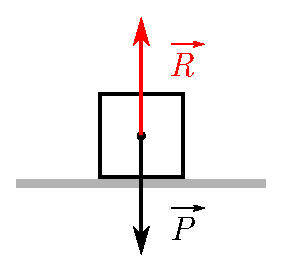
\includegraphics[width=.6\linewidth]{ForceReactionSupport1}
\end{center}
\end{minipage}

\vspace{2em}

\begin{minipage}[c]{.65\linewidth}
Si le support est un plan incliné, deux forces s'appliquent à l'objet : la réaction du support $\vect{R}$ qui empêche l'objet de s'enfoncer dans le support et une \textbf{\MotDefinition{force de frottement}{}} $\vect{f}$ qui empêche l'objet de glisser. La force de frottement a pour droite d'action la parallèle au support et pour sens l'opposé de celui du mouvement (ou du mouvement potentiel) de l'objet.

Notons que si l'objet ne bouge pas (équilibre) $\vect{R_N} + \vect{f} = -\vect{P}$.

\vspace{2em}

\end{minipage}\hfill%
\begin{minipage}[c]{.33\linewidth}
\begin{center}
    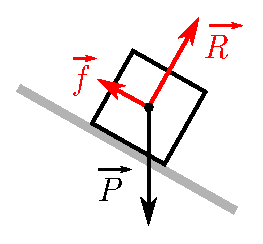
\includegraphics[width=.55\linewidth]{ForceReactionSupport3}
\end{center}
\end{minipage}




\begin{minipage}[c]{.65\linewidth}
Lorsqu'un objet est suspendu à un fil, une \MotDefinition{force de tension}{} $\vect{T}$ apparaît : c'est la force qui retient l'objet et lui évite la chute. La force de tension est toujours dans la même direction que le fil.
\end{minipage}\hfill%
\begin{minipage}[c]{.33\linewidth}
\begin{center}
    \includegraphics[width=.8\linewidth]{ForceTensionFil}
\end{center}
\end{minipage}


Les paragraphes suivants listent les différentes forces rencontrées cette année.

\vspace{1em}

Lorsqu'un objet subit une traction (par exemple par un moteur ou parce qu'on le tire), on parle de \MotDefinition{force de traction}{} ;

\vspace{1em}

Lorsqu'un objet est propulsé (par exemple par un moteur ou encore parce qu'on le pousse), on parle de \MotDefinition{force de propulsion}{} ;

\vspace{1em}

Lorsqu'un objet avance avec une grande vitesse dans l'air ou dans un fluide, des frottements apparaissent : cette \MotDefinition{force de frottement}{} est toujours orientée dans le sens opposé à celui du mouvement et sa droite d'action est celle du déplacement de l'objet ; 

\vspace{1em}

Deux charges électriques de signes opposés s'attirent, de même signe se repoussent : on parle de \MotDefinition{force électrique}{} ;

\vspace{1em}

Un aimant attire les matériaux ferreux : on parle de \MotDefinition{force magnétique}{} ;

\vspace{1em}

Un objet plongé dans un fluide subit une force verticale dirigée vers le haut : la \MotDefinition{poussée d'Archimède}{} (se reporter au chapitre sur pression et hydrostatique).














\connaissances
\begin{acquis}
\begin{itemize}
    \item Définir les termes suivants : action mécanique, force, droite d'action, sens, intensité, point d'application, vecteur, système, acteur, receveur, dynamomètre, newton, résultante des forces
%
    \item Modéliser une action mécanique par une force
%
    \item Décrire quels sont les effets d'une action mécanique
%
    \item Représenter une force par un vecteur en respectant une échelle
%
    \item Identifier, pour une situation donnée, le système, l'acteur, le receveur
%
    \item Citer les caractéristiques d'une force (droite d'action, sens, intensité, point d'application)
%
    \item Établir un diagramme objets--interactions pour une situation donnée
%
    \item Déduire d'un diagramme objets--interactions les forces s'appliquant sur le système étudié
%

    \item Établir graphiquement la somme de plusieurs vecteurs
%
    \item Construire graphiquement la résultante de plusieurs forces, et déterminer son intensité en utilisant une échelle
\end{itemize}
\end{acquis}


\QCMautoevaluation{Pour chaque question, plusieurs réponses sont
  proposées. Déterminer celles qui sont correctes.}

\begin{QCM}
  
  \begin{GroupeQCM}
    
    \begin{exercice}
      La somme de deux forces d'intensité 2\,N est une force d'intensité :
      \begin{ChoixQCM}{4}
      \item $2$\,N
      \item $4$\,N
      \item $0$\,N
      \item on ne peut pas le savoir a priori.
      \end{ChoixQCM}
        \begin{corrige}
        \reponseQCM{d}
        \end{corrige}
    \end{exercice}
    
    
    \begin{exercice}
      Parmi les termes proposés quels sont ceux qui sont équivalents :
      \begin{ChoixQCM}{4}
      \item droite d'action et direction
      \item direction et sens
      \item sens et droite d'action
      \item intensité et valeur
      \end{ChoixQCM}
\begin{corrige}
     \reponseQCM{ad}
   \end{corrige}
    \end{exercice}
    
\end{GroupeQCM}
\end{QCM}



\textbf{TODO : ajouter des exercices "identifier l'action et la réaction", avec par exemple une personne qui pousse un mur, un objet qui tombe, les gaz d'une fusée. Dire qu'elle est l'interaction, quelle est l'action, quelle est la réaction}



\exercicesbase
\begin{colonne*exercice}



\begin{exercice}[]
Compléter le tableau suivant.

\begin{center}
\begin{Ltableau}{\linewidth}{4}{c}
\hline
\textbf{Corps étudié} & \textbf{Receveur} & \textbf{Acteur} & \textbf{Type d'action}  \\ \hline
\includegraphics[angle=0,width=.7cm]{nuagePluie} & Goutte &  &  \\ \hline
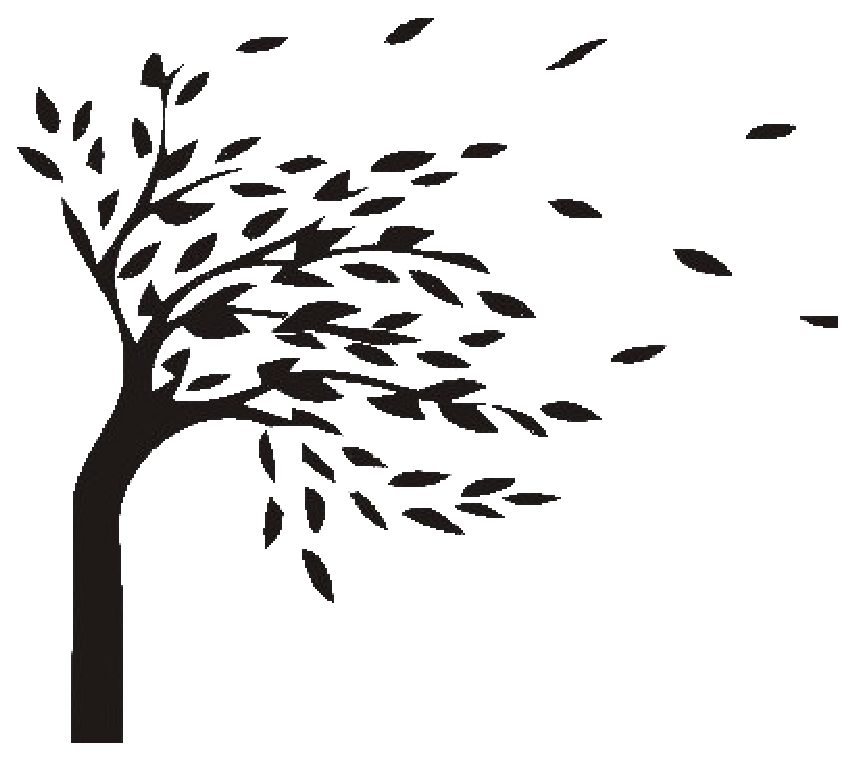
\includegraphics[angle=0,width=1.2cm]{tree} & Feuille & & \\ \hline
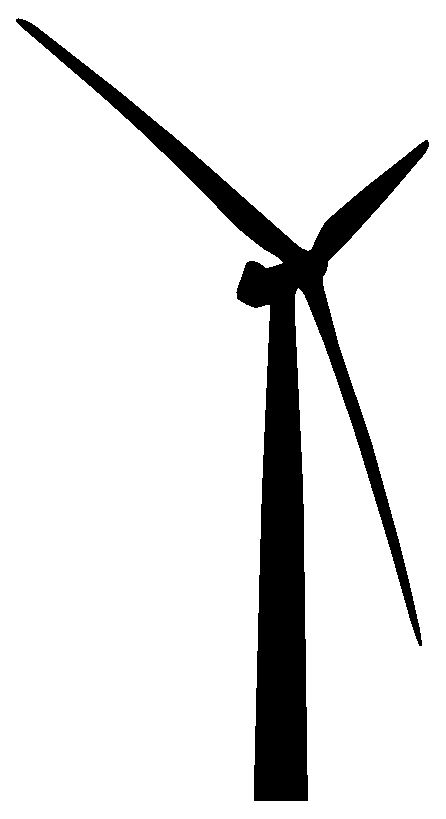
\includegraphics[angle=0,width=.7cm]{eolienne} & Pâle & & \\ \hline
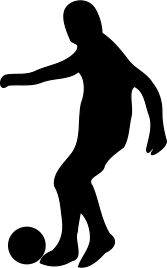
\includegraphics[angle=0,width=.7cm]{footballer} & Ballon & & \\ \hline

\includegraphics[angle=0,width=.7cm]{halterophile} & Homme & & \\ \hline
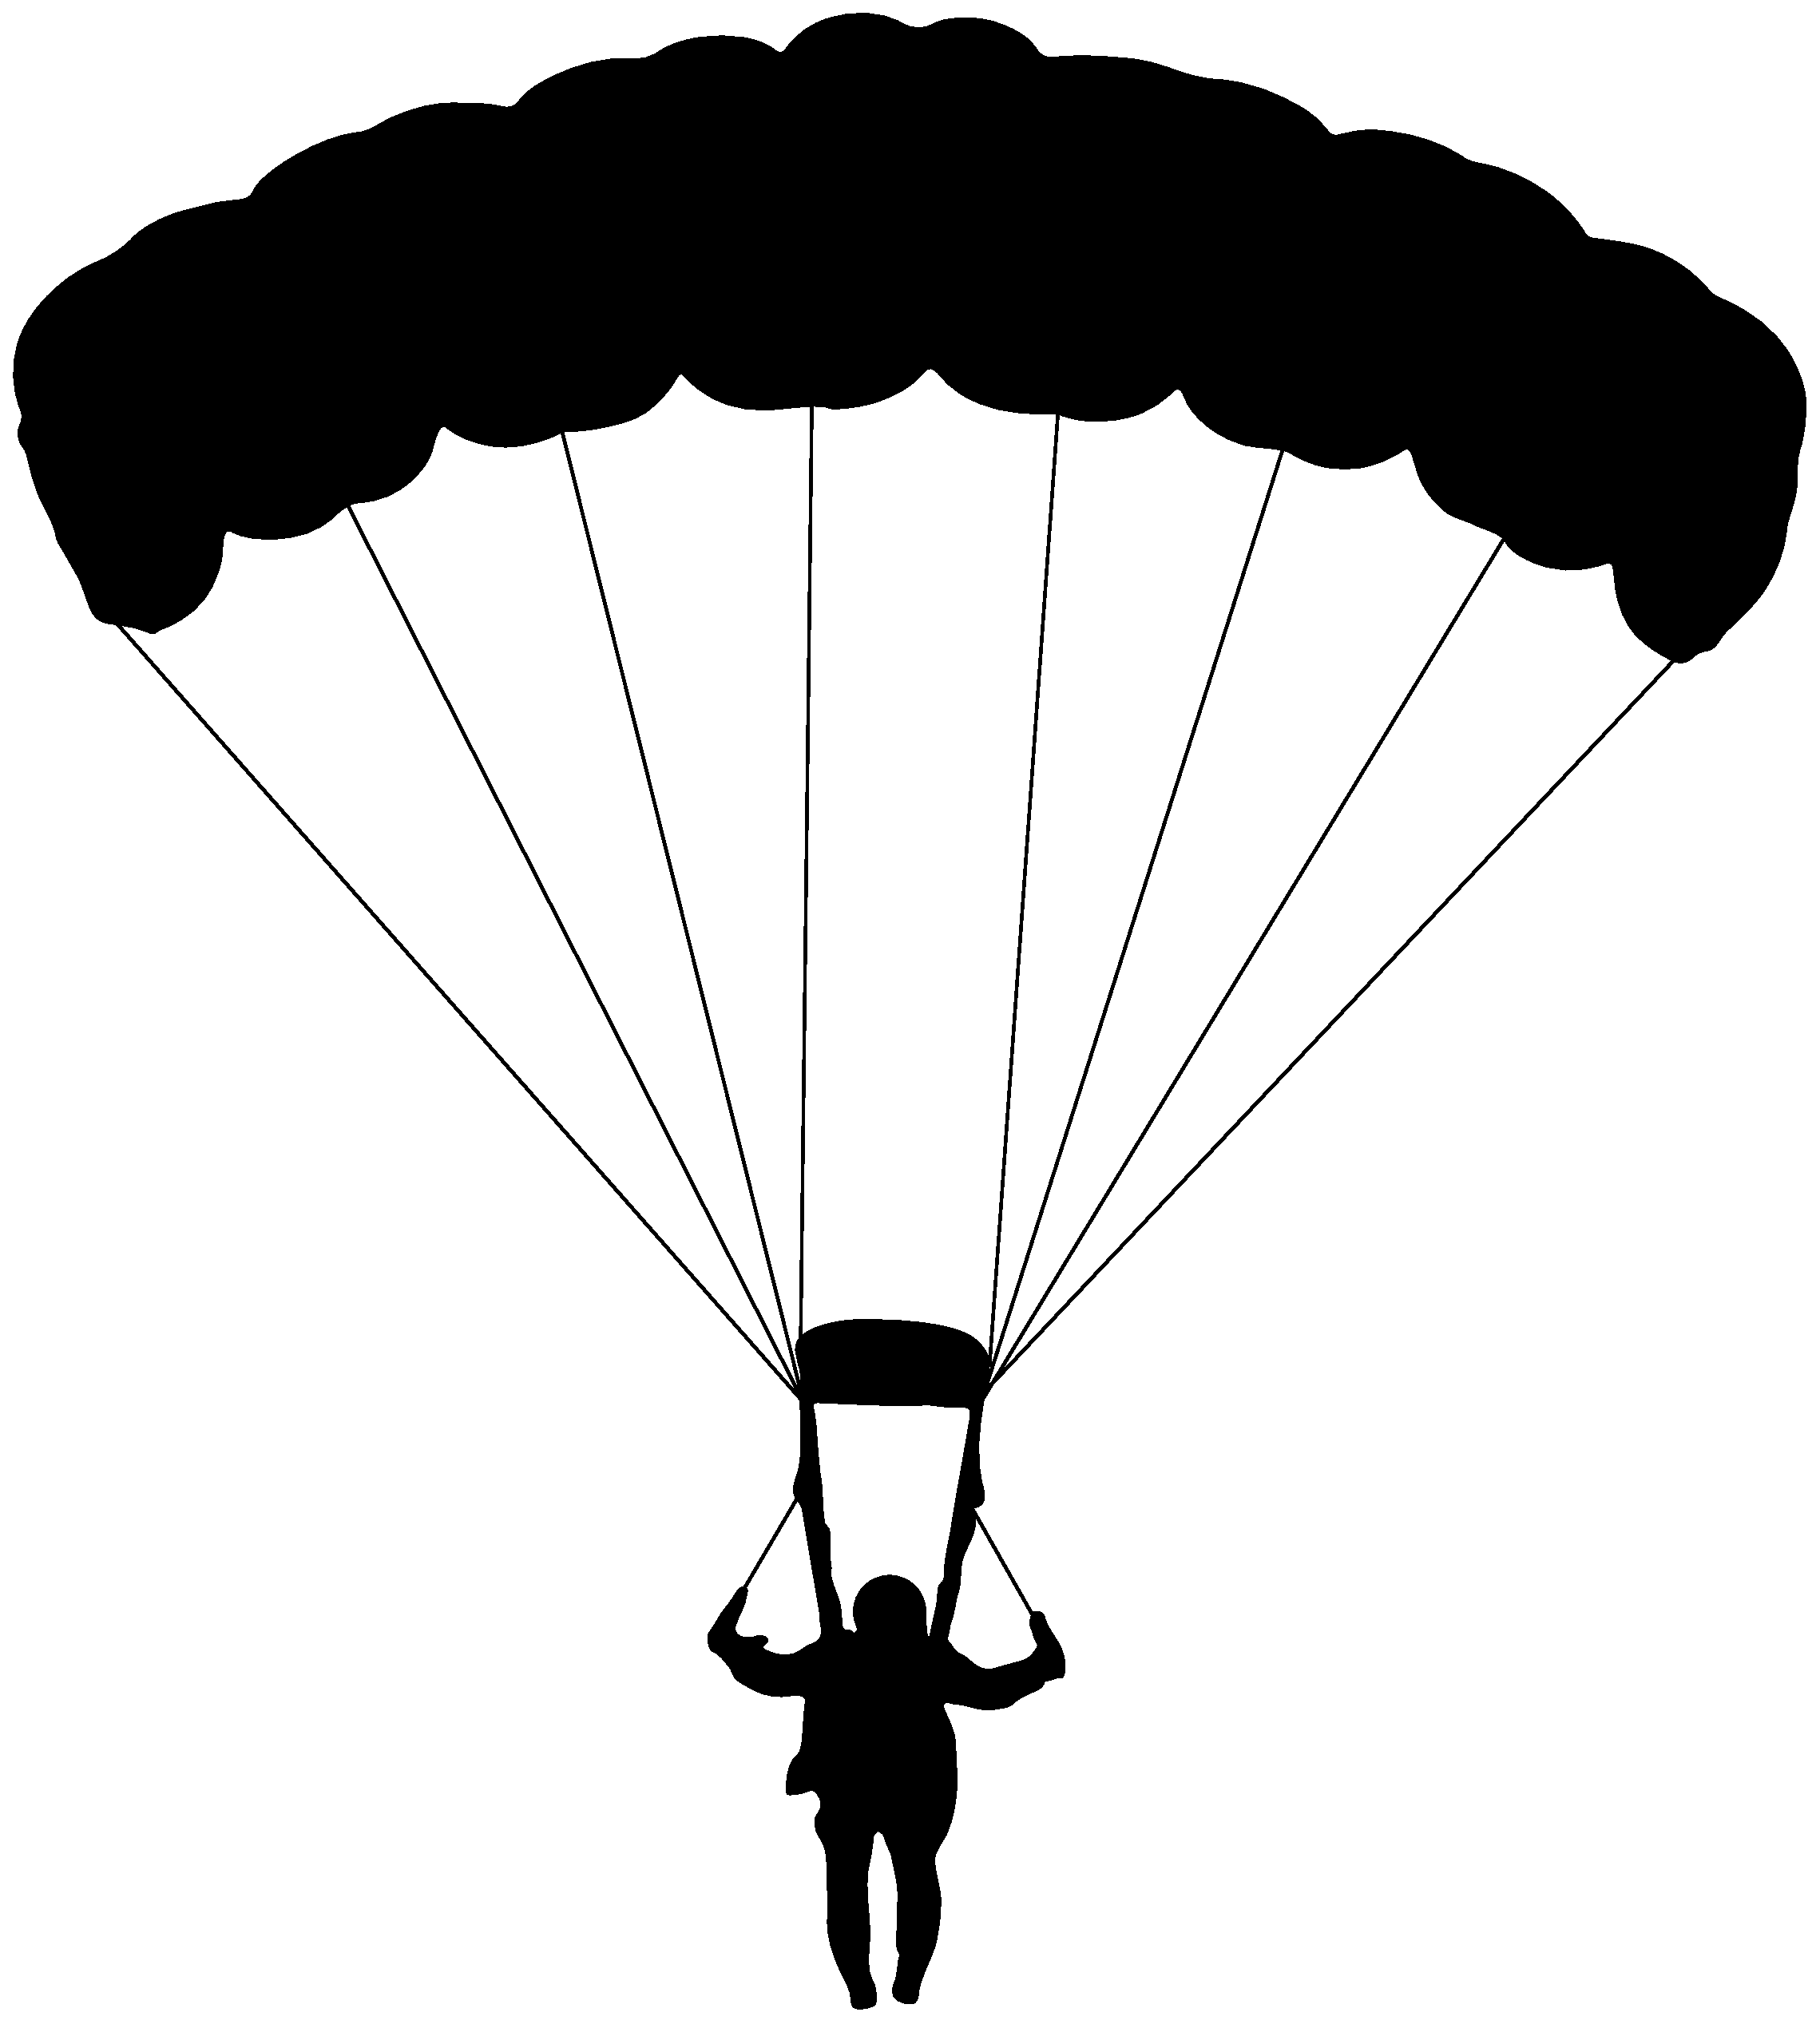
\includegraphics[angle=0,width=1.2cm]{parachute} & Homme & &  \\ \hline
\end{Ltableau}
\end{center}

\end{exercice}

\begin{corrige}
Acteur et receveur

\begin{center}
\begin{Ltableau}{\linewidth}{4}{c}
\hline
\textbf{Corps étudié} & \textbf{Receveur} & \textbf{Acteur} & \textbf{Type d'action}  \\ \hline
\includegraphics[angle=0,width=.4cm]{nuagePluie} & Goutte & Terre & Distance  \\ \hline
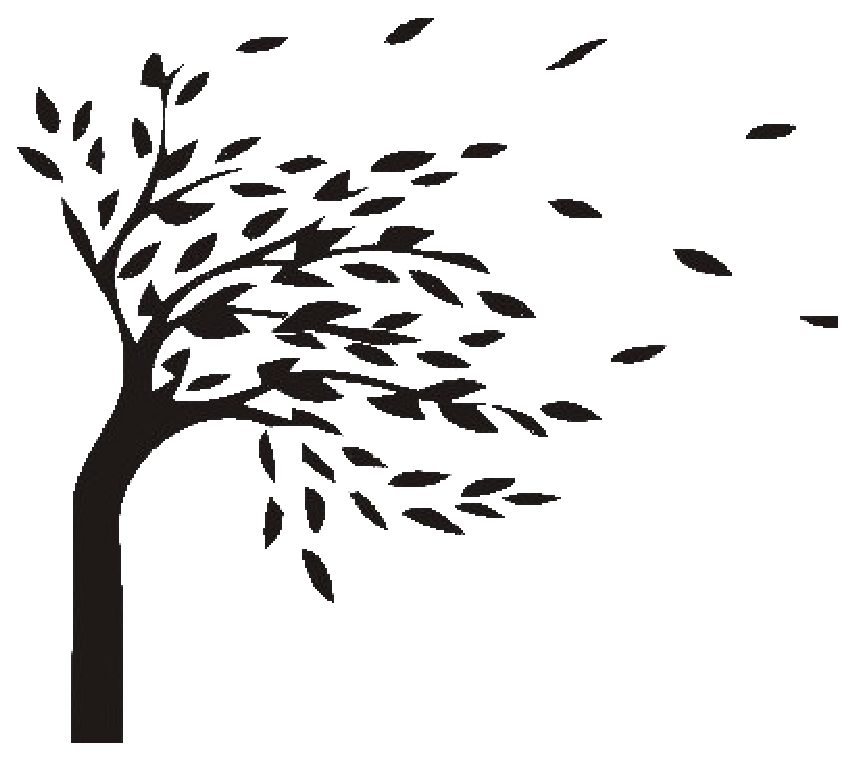
\includegraphics[angle=0,width=.7cm]{tree} & Feuille & Air & Contact \\ \hline
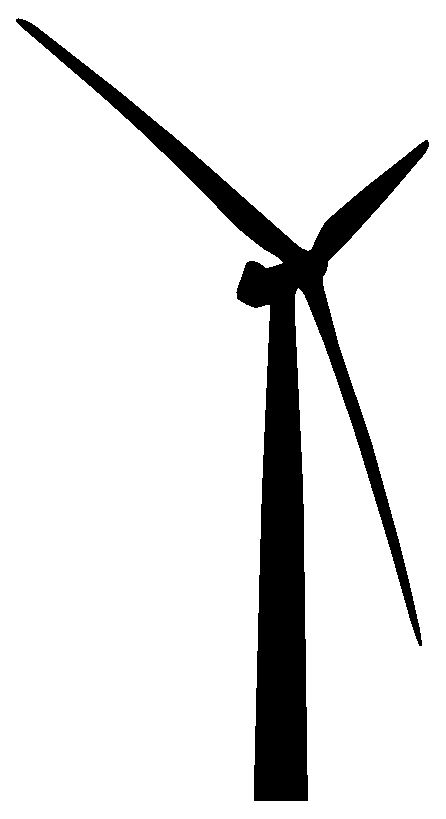
\includegraphics[angle=0,width=.4cm]{eolienne} & Pâle & Air & Contact \\ \hline
\includegraphics[angle=0,width=.4cm]{footballer} & Ballon & Joueur & Contact \\ \hline
\includegraphics[angle=0,width=.4cm]{halterophile} & Homme & Haltères & Contact \\ \hline
\includegraphics[angle=0,width=.7cm]{parachute} & Homme & Parachute & Contact \\ \hline
\end{Ltableau}
\end{center}

\end{corrige}



\begin{exercice}[]\ExerciceRefMethode{methodeForceEchelle}
\label{representeVecteur}

Une personne tire un objet par l'intermédiaire d'une corde. On s'intéresse à la force exercée par la corde sur l'objet. Elle a pour valeur 3\,N.

\vspace{1em}
\begin{center}
    \includegraphics[width=.4\linewidth]{./objetMain}   
\end{center}

\begin{enumerate}
\item Donner toutes les caractéristiques de la force.
\item On prend comme échelle 1\,cm représente 1\,N. Calculer la longueur de la flèche utilisée pour représenter la force.  
\item Représenter, à l'échelle, la force sur le schéma.
\end{enumerate}


\end{exercice}

%\begin{corrige}

%\end{corrige}


% fin de l'exercice


\begin{exercice}
Anaïs tire sur le tendeur avec sa main. Représenter la force exercée par la main ($M$) sur le tendeur ($T$), sachant qu'elle a pour valeur 5\,N. Échelle : 1\,cm pour 2\,N.  

\vspace{1em}
\begin{center}
    \includegraphics[width=.4\linewidth]{./tendeurMain}   
\end{center}

\end{exercice}

%\begin{corrige}
%Tendeur et main

%\end{corrige}





\begin{exercice}
Au service, la force $\vect{F_1}$ exercée par la raquette d'un joueur de tennis sur la balle vaut 1200\,N. Sur le schéma, on a représenté en pointillé la ligne d'action des forces. Représenter $\vect{F_1}$ à l'échelle 1\,cm pour 500\,N.

\vspace{1em}
\begin{center}
    \includegraphics[width=.4\linewidth]{./tennisBall}   
\end{center}

\end{exercice}

%\begin{corrige}
%Service au tennis

%\end{corrige}


















\begin{exercice}
Répondre aux questions suivantes sur les forces.
\begin{enumerate}
\item Avec quel appareil mesure-t-on l'intensité d'une force ?
\item Quelle est l'unité légale de force ?
\item Quel est son symbole ?
\end{enumerate}
\end{exercice}


\begin{corrige}
\begin{enumerate}
\item L'intensité d'une force se mesure grâce à un dynamomètre.
\item L'unité légale de la force est le newton.
\item Symbole du newton : N.
\end{enumerate}
\end{corrige}






\begin{exercice}
Répondre aux questions suivantes sur les forces.
\begin{enumerate}
\item Que modélisent les forces ? 
\item Quelles sont les quatre caractéristiques d'une force ?
\item Par quoi est représentée une force ?
\end{enumerate}
\end{exercice}


\begin{corrige}
\begin{enumerate}
\item Les forces modélisent des actions mécaniques.
\item Les quatre caractéristiques sont : droite d'action (direction), sens, intensité, point d'application.
\item Une force est représentée par un vecteur.
\end{enumerate}
\end{corrige}






\begin{exercice}
Dire si les propositions suivantes sont vraies ou fausses. Corriger celles qui sont fausses.
\begin{enumerate}
\item Les actions de contact peuvent être ponctuelles ou réparties.
\item L'action du vent sur la voile du véliplanchiste est une action à distance.
\item L'unité légale de la force est le kilogramme, de symbole kg.
\item La valeur d’une force se mesure avec un dynamomètre.
\end{enumerate}
\end{exercice}


\begin{corrige}
\begin{enumerate}
\item Vrai 
\item Faux (contact entre l'air et la voile)
\item Faux, c'est le newton (N).
\item Vrai
\end{enumerate}
\end{corrige}








\begin{exercice}
Observer la figure ci-dessous.

\begin{minipage}[c]{.28\linewidth}
\centering
\includegraphics[width=.8\linewidth]{pommeDynamo}
\end{minipage}\hfill%
\begin{minipage}[c]{.68\linewidth}
\begin{enumerate}
\item Quel est le nom de l'appareil de mesure ?
\item En quelle unité est-il gradué ?
\item Quelle est la valeur de la force ? 
\end{enumerate}
\end{minipage}
\end{exercice}


\begin{corrige}
\begin{enumerate}
\item L'appareil est un dynamomètre.
\item Il est gradué en newton.
\item Par lecture graphique, on trouve $F=2$\,N. 
\end{enumerate}
\end{corrige}








\begin{exercice}
Indiquer si les actions mécaniques suivantes sont des actions de contact ou des actions à distance :
\begin{enumerate}
\item action du marteau sur le clou ;
\item action du pied sur le ballon ;
\item action de l'aimant sur la bille de fer ;
\item action du vent sur le cerf-volant ;
\item action de la Lune sur les océans.
\end{enumerate}
\end{exercice}


\begin{corrige}
\begin{enumerate}
\item Marteau et clou : action de contact.
\item Pied et ballon : action de contact.
\item Aimant et bille : action à distance.
\item Vent et cerf-volant : action de contact.
\item Lune et océan : action à distance.
\end{enumerate}
\end{corrige}















\begin{exercice}
Sachant que l'intensité de la force $\vect{F}$ est de 100\,N, donner toutes les caractéristiques de la force ainsi que l'échelle utilisée pour la représenter.

\vspace{1em}
\begin{center}
    \includegraphics[width=.15\linewidth]{cubeCable}
\end{center}

\end{exercice}


\begin{corrige}
\begin{enumerate}
\item Force : $F$ (tension du fil).
\item Point d'application : jonction entre corde et solide.
\item Droite d'action : la corde.
\item Sens : de bas en haut.
\item Intensité : $F=100$\,N. 
\end{enumerate}
\end{corrige}







\begin{exercice}
Un marteau exerce une force sur un clou. Sachant que l'intensité de la force $\vect{F}$ est de 50\,N, donner toutes les caractéristiques de la force puis la représenter en utilisant l'échelle 1\,cm pour 25\,N.

\vspace{1em}
\begin{center}
    \includegraphics[width=.4\linewidth]{marteauClou}
\end{center}

\end{exercice}


\begin{corrige}
\begin{enumerate}
\item Force : $F$ (appui du marteau sur le clou).
\item Point d'application : tête du clou.
\item Droite d'action : droite matérialisée par le clou.
\item Sens : de haut en bas.
\item Intensité : $F=50$\,N. 
\end{enumerate}

\begin{center}
    \includegraphics[width=.4\linewidth]{marteauClouCorrection}
\end{center}

\end{corrige}








\begin{exercice}
Une personne pousse un wagonnet comme indiqué sur le schéma ci-dessous, avec une force d'intensité 500\,N. Donner les caractéristiques de la force puis la représenter à l'échelle 1\,cm représente 200\,N.

\vspace{1em}
\begin{center}
    \includegraphics[width=.5\linewidth]{wagonnet}
\end{center}

\end{exercice}


\begin{corrige}
\begin{enumerate}
\item Force : $F$ (action de l'homme sur le wagonnet).
\item Point d'application : point de contact main--wagonnet.
\item Droite d'action : droite parallèle aux rails, passant par les mains.
\item Sens : de l'homme vers le wagonnet.
\item Intensité : $F=500$\,N. 
\end{enumerate}

\vspace{1em}

\begin{center}
   \includegraphics[width=.6\linewidth]{wagonnetCorrection}
 
\end{center}

\end{corrige}


\begin{exercice}\ExerciceRefMethode{methodeAddBoutBout} ou \ExerciceRefMethode{methodeAddParall}
\label{exAddVect}

Pour chacun des cas ci-dessous, indiquer les sommes vectorielles $\vec{a}+\vec{b}$ qui sont correctes et celles qui sont incorrectes.

\vspace{1em}
\begin{center}
    \includegraphics[width=\linewidth]{./sommeVecteurs}   
\end{center}

\end{exercice}





\begin{corrige}
Sommes vectorielles : vrai ou faux ?

\begin{center}
    \includegraphics[width=\linewidth]{./sommeVecteursCorrection}   
\end{center}

\end{corrige}








\begin{exercice}
Pour chacun des cas ci-dessous, tracer graphiquement la somme des deux vecteurs $\vect{a}$ et $\vect{b}$.

\vspace{1em}
\begin{center}
    \includegraphics[width=\linewidth]{./sommeVecteurs2}   
\end{center}

\end{exercice}


\begin{corrige}
Sommes vectorielles

\begin{center}
    \includegraphics[width=\linewidth]{./sommeVecteurs2Correction}   
\end{center}

\end{corrige}





\begin{exercice}
Dans chacun des cas ci-dessous, un solide est soumis à deux forces $\vec{f_1}$ et $\vec{f_2}$. Tracer à chaque fois la résultante de ces forces, et donner son intensité (échelle : 1\,cm pour 1\,N).

\vspace{1em}
\begin{center}
    \includegraphics[width=.8\linewidth]{./forcesSolide}   
\end{center}

\end{exercice}


\begin{corrige}
Solide soumis à deux forces

\begin{center}
    \includegraphics[width=\linewidth]{./forcesSolideCorrection}   
\end{center}

Dans chacun des cas, on mesure la résultante et, en utilisant l'échelle, on obtient l'intensité (indiquée en dessous de chaque figure).
\end{corrige}




\begin{exercice}
Un hors-bord tracte deux skieurs nautiques. Chacun d'eux exerce sur le hors-bord une force de valeur 500\,N.

\vspace{1em}
\begin{center}
    \includegraphics[width=.7\linewidth]{./bateauSki}   
\end{center}


\begin{enumerate}
\item Représenter cette force en utilisant l’échelle 1 cm représente 100 N.
\item Déterminer graphiquement la somme (la résultante) de ces deux forces.
\item Déterminer l'intensité de la résultante.
\end{enumerate}
\end{exercice}


\begin{corrige}
Hors-bord

\begin{center}
    \includegraphics[width=\linewidth]{./bateauSkiCorrection}   
\end{center}

La résultante est mesurée une fois tracée. Elle mesure 9\,cm, soit une intensité de 900\,N (échelle 1\,cm pour 100\,N).    
\end{corrige}





\begin{exercice}
En utilisant deux vecteurs $\vec{u}$ et $\vec{v}$, montrer que $\vec{u} + \vec{v} = \vec{v} + \vec{u}$.
\end{exercice}


\begin{corrige}
Pour cela on trace $\vec{u} + \vec{v}$ puis $\vec{v} + \vec{u}$ :

\vspace{1em}
\begin{center}
    \includegraphics[width=.4\linewidth]{./somme_u_v}   
\end{center}

Graphiquement, on constate que quelque soit l'ordre d'addition, on obtient la même somme vectorielle $\vec{u} + \vec{v}$.
\end{corrige}



\begin{exercice}
Une bille en train de chuter dans l'air est soumise à deux forces (figure ci-dessous).
\vspace{1em}
\begin{center}
    \includegraphics[width=.15\linewidth]{bouleForces}   
\end{center}
%
\begin{enumerate}
\item $\vect{F_1}$ représente une force ; laquelle ?
\item $\vect{F_2}$ représente une force ; laquelle ?
\end{enumerate}

\end{exercice}

\begin{corrige}
\begin{enumerate}
\item $\vect{F_1}$ représente les frottements de l'air qui freinent la bille.
\item $\vect{F_2}$ représente le poids de la bille (dû à la gravité terrestre).
\end{enumerate}
\end{corrige}







\begin{exercice}
Les remorqueurs 1 et 2 tirent une barge, générant une force de tension dans chaque câble $AB$ et $AC$. La tension du câble $AB$ a pour intensité $T_1 = 85$\,kN, celle du câble $AC$, $T_2 = 13$\,kN.
\begin{enumerate}
\item Quelle interaction est modélisée par la force $T_1$ ?
\item Par quel objet est représentée la force $T_1$ ?
\item Donner les caractéristiques de la force de tension $T_1$.
\item Choisir une échelle, tracer au point $A$ la résultante $R$ des forces $T_1$ et $T_2$.
\item Déterminer graphiquement l'intensité de $R$.
\end{enumerate}
\vspace{1em}
\begin{center}
    \includegraphics[width=.7\linewidth]{./barge}   
\end{center}

\end{exercice}

\begin{corrige}
\begin{enumerate}
\item L'interaction modélisée par la force $T_1$ est la traction exercée par le remorqueur 1 sur le câble.
\item La force $T_1$ est représentée par un vecteur : $\vect{T_1}$.
\item Les caractéristiques de la force $\vect{T_1}$ sont : direction $(AB)$, sens de $A$ vers $B$, intensité de 85\,kN et point d'application $A$.
\item On choisit comme échelle 1\,cm représente 12\,kN. (Pour trouver l'échelle, on prend la plus grande intensité à représenter, 85\,kN ici, et la place disponible pour la représenter sur $(AB)$, 7\,cm ici. Ainsi, par proportionnalité, 1\,cm représente 12,1\,kN, que l'on arrondit à 1\,cm pour 12\,kN).
La force $\vect{T_1}$ est donc représentée par 7,1\,cm et la force $\vect{T_2}$ par 1,1\,cm.

\includegraphics[width=.8\linewidth]{./exerciceBargeCorr}   

\item Sur le graphique, la résultante $\vect{R}$ est représentée par 7,5\,cm. Son intensité est donc de 90\,kN.
\end{enumerate}
\end{corrige}


% ex DOI


 \serie{Diagramme objets--interactions}

Pour les exercices \RefExercice{doiFirst} à \RefExercice{doiLast} établir un diagramme objets--interactions et en déduire le nombre de forces appliquées au système (le système étudié est indiqué en dessous de la figure).

\begin{exercice}\ExerciceRefMethode{methodeDOI}
\label{doiFirst}
\begin{center}
    \includegraphics[width=.2\linewidth]{./pendule}  
    
    Bille
\end{center}
\end{exercice}

\begin{corrige}
Bille

\begin{center}
    \includegraphics[width=\linewidth]{./doiBille}  
\end{center}
Il y a deux interactions dans le DOI donc le système est soumis à deux forces : l'attraction gravitationnelle de la Terre et la force de tension du fil qui retient la bille. L'action de l'air est négligée car la bille n'est pas en mouvement et sa masse volumique est bien plus grande que celle de l'air.
\end{corrige}

\begin{exercice}
\begin{center}
    \includegraphics[width=.4\linewidth]{./patinGlace}   
    
    Patineuse qui avance lentement
\end{center}
\end{exercice}

\begin{corrige}
Patineuse

\begin{center}
    \includegraphics[width=\linewidth]{./doiPatineuse}  
\end{center}
Il y a deux interactions dans le DOI donc le système est soumis à deux forces : l'attraction gravitationnelle de la Terre et la réaction du support. L'action de l'air est négligée car la patineuse avance lentement et sa masse volumique est bien plus grande que celle de l'air.
\end{corrige}

\begin{exercice}
\begin{center}
    \includegraphics[width=.5\linewidth]{./voiturePente} 
    
    Voiture arrêtée dans une pente
\end{center}
\end{exercice}

\begin{corrige}
Voiture

\begin{center}
    %\includegraphics[width=\linewidth]{./doiVoiture}  
\end{center}
\end{corrige}

\begin{exercice}
\begin{center}
    \includegraphics[width=.2\linewidth]{./parachute} 
    
    Parachutiste et son matériel
\end{center}
\end{exercice}



\begin{exercice}
\begin{center}
    \includegraphics[width=.3\linewidth]{./moto}
    
    Moto qui roule vite
\end{center}
\end{exercice}



\begin{exercice}\label{doiLast}
\begin{center}
    \includegraphics[width=.2\linewidth]{./montgolfiere}
    
    Montgolfière qui se déplace avec la masse d'air
\end{center}
\end{exercice}



























































\end{colonne*exercice}






% début des annexes
\annexe{La démarche scientifique}

\begin{center}
    \vfill
    \includegraphics[width=.6\linewidth]{demScientifiqueScience}
    \vfill
\end{center}
\annexe{Les critères d'évaluation}

\vspace{3em}
%%%%%%%%%%%%%%%%%%%%%%%%%%%%%%%%%%%%%%%%%%%%%%%%%%%%%%%%%%%%%%%%%
%                   TABLEAU CRITÈRES
\begin{center}
{\footnotesize % fin du footnotesize 11 lignes plus bas
\definecolor{gris}{rgb}{.7,.7,.7}
\begin{tabularx}{.7\linewidth}{|l|X|c|c|}
\cline{3-4}
\multicolumn{2}{l|}{} & {\scriptsize Points obtenus} & {\scriptsize Total des points}    \\ \hline
Critère A   & \textsl{Connaissance et compréhension} & & \\ \hline
Critère B   & Démarche scientifique : \textsl{Recherche et élaboration}      & & \\ \hline
Critère C   & \textsl{Communication}                 & & \\ \hline
Critère D   & Démarche scientifique : \textsl{Traitement et évaluation}      & & \\ \hline
\multicolumn{2}{l|}{}   & \cellcolor{gris} & \cellcolor{gris} \\ \cline{3-4}
\end{tabularx}
} % fin du footnotesize
\end{center}
%
%%%%%%%%%%%%%%%%%%%%%%%%%%%%%%%%%%%%%%%%%%%%%%%%%%%%%%%%%%%%%%%%%



\section{Critère A (Connaissance et compréhension)}

L'élève est capable :
\begin{itemize}
\item de répondre à des questions de cours, de citer des définitions, de refaire un schéma ;
\item d’expliquer des connaissances scientifiques ;
\item d’appliquer des connaissances et une compréhension scientifiques pour résoudre des problèmes tirés de situations aussi bien familières que nouvelles ;
\item d’analyser et d’évaluer des informations afin de formuler des jugements scientifiquement étayés.
\end{itemize}


\section{Critère B (Démarche scientifique : recherche et élaboration)}

L'élève est capable :
\begin{itemize}
\item d’expliquer un problème ou une question qui sera vérifié(e) par une recherche scientifique ;
\item de formuler une hypothèse vérifiable et de l’expliquer en faisant appel à un raisonnement scientifique ;
\item d’expliquer la façon de manipuler les variables et d’expliquer la manière dont les données seront recueillies ;
\item d’élaborer des recherches scientifiques.
\end{itemize}



\section{Critère C (Communication)}

L'élève est capable :
\begin{itemize}
\item de rendre compte de façon écrite, de manière synthétique et structurée, en utilisant un vocabulaire adapté, une langue correcte et précise ;
\item de rendre compte de façon orale, de résumer sa démarche, de transmettre l’information de manière synthétique et claire, de s’exprimer à l’oral avec aisance ;
\item d'utiliser un langage scientifique de manière correcte et efficace ;
\item de présenter des résultats avec l'outil informatique ;
\item de documenter les travaux d’autrui et les sources d’information utilisées.
\end{itemize}


\section{Critère D (Démarche scientifique : traitement et évaluation)}

L'élève est capable :
\begin{itemize}
    \item de présenter des données recueillies et transformées ;
    \item d’interpréter des données et d’expliquer des résultats en faisant appel à un raisonnement scientifique ;
    \item d’évaluer la validité d’une hypothèse en fonction du résultat de la recherche scientifique ;
    \item d’évaluer la validité de la méthode employée ;
    \item d’expliquer des moyens d’améliorer ou d’approfondir la méthode.
\end{itemize}







\annexe{Concevoir une expérience}

Le but est d'effectuer une \textbf{démarche scientifique} : \newline
(i) Formuler un problème, une question de recherche, (ii) Émettre une hypothèse et prévoir les conséquences observables, (iii) Tester l'hypothèse par l'expérimentation (concevoir une expérience), (iv) Confronter les résultats à la prévision, (v) Conclure (l'hypothèse est validée, l'hypothèse est confortée, l'hypothèse est rejetée).

\section{Définir le problème et sélectionner les variables}  


\begin{enumerate}
\item Définir la \textbf{question de recherche} : c'est le problème sur lequel vous allez travailler. L'hypothèse (voir plus bas) est une réponse possible à cette question. La vraie réponse sera donnée dans la conclusion.
%
\item Définir quelle sera la \underline{variable indépendante} et préciser son unité. C'est la variable, le paramètre, que vous allez faire varier dans votre expérience (cause).
%
\item Définir quelle sera la \underline{variable dépendante} et préciser son unité. C'est la variable, le paramètre, que vous allez mesurer dans votre expérience (effet).
%
\item Lister ce que vous savez déjà sur le sujet : recherches effectuées, connaissances personnelles, observations déjà effectuées, premiers essais. Ceci doit vous permettre de formuler une hypothèse de recherche valable.
%
\item Écrire une \textbf{hypothèse} pour votre expérience, basée sur ce que vous savez déjà. L'hypothèse est une \textbf{prédiction du résultat de l'expérience}. Les variables indépendante et dépendante doivent clairement apparaître dans l'hypothèse. L'hypothèse doit pouvoir être testée et vérifiée par l'expérience.
%
\item Précisez et détaillez comment sont mesurées les variables indépendante et dépendante.
%
\item Identifier les \underline{variables contrôlées} et leurs effets possibles sur les résultats. Ce sont les variables, les paramètres de l'expérience, qui doivent rester constants afin de ne pas fausser les résultats. Décrire quelles seront vos actions permettant de contrôler ces variables. 
%
\item Proposer une \textbf{expérience}. Détailler pas à pas les étapes à réaliser pour mener à bien votre expérience (première version du protocole d'expérience). Les étapes doivent être suffisamment claires pour permettre à une autre personne de réaliser la même expérience. Lister précisément le matériel et les produits nécessaires. Remarque : c'est quand vous rédigerez votre compte rendu, une fois l'expérience réalisée, que vous rédigerez la version finale du protocole d'expérience.
%
\end{enumerate}

\section{Avant de collecter les données}

\begin{enumerate}
%
\item Assurez-vous que suffisamment de données seront collectées (quel volume de données est nécessaire pour valider votre hypthèse ?).
\item Combien de fois seront répétées les mesures afin de s'assurer de la reproductibilité des résultats et améliorer leur précision ?
\item Préparer un grand tableau pour y consigner les résultats bruts. Écrire un titre descriptif au sommet de chaque tableau. Numéroter chacun des tableaux, afin de pouvoir s'y référer (\emph{<<\,voir tableau \no 1\,>>}). Inclure les unités et les incertitudes de mesure pour chaque colonne dans les tableaux de données.
\item Faire un schéma ou prendre une photographie du montage utilisé. Légender tout l'équipement et le matériel utilisés.
\end{enumerate}





\section{Traiter les données}

\textsl{Le traitement des données inclut tous les calculs ou manipulations réalisés sur les données brutes : calculs variés, réalisation de graphiques, etc. En général, la variable indépendante est représentée en abscisse et la variable dépendante en ordonnée.}

\begin{enumerate}
\item Inclure un exemple de chaque calcul effectué sur les données bruts (vérifier les calculs pour éviter les erreurs !).
\item Présenter les résultats traités sous forme de feuille de calculs, tableaux, graphiques, illustrations, diagrammes, etc.
\item Les graphiques doivent être précis et posséder des étiquettes d'axes avec unités.
\item Sous chaque graphique, illustration, diagramme, etc., inclure une numérotation (permettant de s'y référer) et un titre qui décrit ce qui est présenté.

\item Les valeurs numériques doivent être présentés avec une unité, un nombre de chiffres significatifs adaptés et une incertitude lorsque cela est pertinent.
\end{enumerate}




\section{Apporter une réponse}

\textsl{Vous devez apporter une réponse à votre question de recherche.}


\begin{enumerate}
\item Interprétez vos résultats : quelle est la réponse à votre problème ? Relisez votre hypothèse et comparez votre réponse à ce que vous aviez prévu. Les données collectées sont-elles en accord avec vos hypothèses ? Pourquoi ou pourquoi pas ?

\item Vos résultats sont-ils fiables ? Y a-t-il des résultats anormaux ? Quelle peut en être la cause ou la signification ?

\item Comparez vos résultats à d'autres sources de données ou d'informations (citez les sources). Calculez l'écart en pourcent entre vos valeurs et celles de la littérature. Tirez une conclusion.

\end{enumerate}



\section{Évaluation et amélioration}

\begin{enumerate}
\item Avez-vous rencontrer des problèmes lors de vos expériences ? Comment ont-ils affecté vos résultats ? Qu'avez-vous fait pour limiter leurs impacts sur les résultats ?

\item Quels sont les points faibles de votre protocole et comment ont-ils pu affecter vos résultats ? Pour chaque point faible ou limitation mentionné, proposez une solution ou des pistes d'amélioration.

\item Est-ce que quelque chose pouvant affecter la fiabilité de vos résultats est arrivé durant vos expériences ?

\item Comment pourriez-vous améliorer, développer ou approfondir cette recherche en vue d'une étude future ?
\end{enumerate}

\vspace{1em}
Pour rédiger le compte rendu, vous pouvez utiliser la fiche méthode \emph{Rédiger un compte rendu d'expérience}. 

{\huge todo : faire un lien avec la fiche dem sciQ et la fiche rédiger comt-rendu}


\AfficheListeMethodes
\AfficheCorriges[2]
\AfficheLexique

\end{document}


% todo
% ajouter des exercices sans calculatrice, unité, dém sc, etc. pour chaque chapitre.
